\documentclass[12pt, titlepage]{article}

\usepackage{fullpage}
\usepackage[round]{natbib}
\usepackage{multirow}
\usepackage{booktabs}
\usepackage{tabularx}
\usepackage{graphicx}
\usepackage{float}
\usepackage{hyperref}
\hypersetup{
    colorlinks,
    citecolor=blue,
    filecolor=black,
    linkcolor=red,
    urlcolor=blue
}

%% Comments

\usepackage{color}

\newif\ifcomments\commentstrue %displays comments
\newif\ifcomments\commentsfalse %so that comments do not display

\ifcomments
\newcommand{\authornote}[3]{\textcolor{#1}{[#3 ---#2]}}
\newcommand{\todo}[1]{\textcolor{red}{[TODO: #1]}}
\else
\newcommand{\authornote}[3]{}
\newcommand{\todo}[1]{}
\fi

\newcommand{\wss}[1]{\authornote{blue}{SS}{#1}} 
\newcommand{\plt}[1]{\authornote{magenta}{TPLT}{#1}} %For explanation of the template
\newcommand{\an}[1]{\authornote{cyan}{Author}{#1}}

%% Common Parts

\newcommand{\progname}{Sayyara} % PUT YOUR PROGRAM NAME HERE
\newcommand{\authname}{Team 31
\\ SFWRENG 4G06
\\ Christopher Andrade
\\ Alyssa Tunney
\\ Kai Zhu
\\ Ethan Vince-Budan
\\ Collin Kan
\\ Harsh Gupta} % AUTHOR NAMES                  

\usepackage{hyperref}
    \hypersetup{colorlinks=true, linkcolor=blue, citecolor=blue, filecolor=blue,
                urlcolor=blue, unicode=false}
    \urlstyle{same}

\newcounter{acnum}
\newcommand{\actheacnum}{AC\theacnum}
\newcommand{\acref}[1]{AC\ref{#1}}

\newcounter{ucnum}
\newcommand{\uctheucnum}{UC\theucnum}
\newcommand{\uref}[1]{UC\ref{#1}}

\newcounter{mnum}
\newcommand{\mthemnum}{M\themnum}
\newcommand{\mref}[1]{M\ref{#1}}

\begin{document}

\title{System Design for \progname{}} 
\author{\authname}
\date{\today}

\maketitle

\pagenumbering{roman}

\section*{Revision History}

\begin{table}[H]
    \begin{tabularx}{\textwidth}{p{3cm}p{2cm}X}
        \toprule {\bf Date} & {\bf Version} & {\bf Notes}\\
        \midrule
        Jan. 18, 2023 & Rev 0 & Revision 0 \\
        April 5, 2023 & Rev 1 & Revision 1 \\
        \bottomrule
    \end{tabularx}
    \caption{Revision History}
\end{table}

\newpage

\section*{Reference Material}

\subsection*{Abbreviations and Acronyms}

\renewcommand{\arraystretch}{1.2}
\begin{table}[H]
    \begin{tabular}{l l} 
      \toprule		
      \textbf{symbol} & \textbf{description}\\
      \midrule 
      \progname & Explanation of program name\\
      UI & User interface - the visual part of the application end users will see \\
      \bottomrule
    \end{tabular}
    \caption{Abbreviations and Acronyms}
\end{table}

\newpage

\tableofcontents

\newpage

\listoftables

\listoffigures

\newpage

\pagenumbering{arabic}

\section{Introduction}
% A]yssa

The system design document outlines more of a general overview of the system and how it connects to the requirements documented in the SRS. More specific, in-depth details of planned system design can be found in the Module Guide and Module Interface Specification documents to supplement the information displayed in this document. Sections with N/A were omitted due to not being suited for the type of project that is being developed.

\section{Purpose}
% A]yssa

The purpose of the Sayyara system is to introduce a solution for both customers and shops in the automotive industry. The application will serve as a hub for customers to submit requests and schedule appointments with automotive shops and shop employees will be able to maintain an online presence for their business. The purpose of the system design document is to outline the overall components of the Sayyara application and display how the design is connected to the requirements documented in the SRS. This document serves as the basis for the how the team is currently implementing requirements and plans to implement the rest of the requirements into the Sayyara application.

\section{Scope}
\begin{figure}[H]
    \centering
    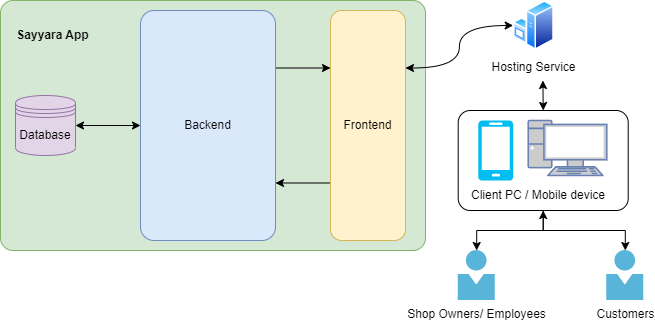
\includegraphics[scale=0.6]{Design/SystDesign/scope.png}
    \caption{The system is defined as the Sayyara App, which includes the backend, frontend, and data storage of the application. Hosting services and client devices are outside the boundary of the system}
    \label{fig:scope}
\end{figure}

\section{Project Overview}

Sayyara is a tech platform that seeks to improve customer acquisition for automotive shops by creating a digital storefront. The Sayyara application is designed to streamline the workflow of the shop by allowing customers to submit quotes and take appointments through desktop and mobile devices. The shop owners are able to easily set up their digital storefront, and their employees can quickly access the tools they need to respond to customer inquiries and schedule appointments. Customers are able to filter through automotive shops in their area by the type of service provided, location, etc. This creates an efficient and transparent communication platform between customers and automotive shops, a revenue booster for shops, and a more understandable, accessible scheduling tool for shop employees.

\subsection{Normal Behaviour}
The normal behaviour for Sayyara is a function of the roles of customers, shop owners, and employees.

\begin{itemize}
    \item Customers can use the Sayyara application to submit quotes requests. They are able to filter through shops in their area by service type and location. They can easily submit quote requests to any shop they choose and are able to track their appointment status through the application. 

    \item Shop Owners are able to set up their digital storefront, as well as customize the services they offer, the shop capacity, and the scheduling. They can easily manage their customer base, respond to customer inquiries and quotes requests, and track their revenue in the application.

    \item Employees are only able to sign up through a special link setup for their specific shop. They have access to the tools they need to respond to customer inquiries and schedule appointments. The application also keeps track of their daily, weekly, and monthly performance metrics and allows them to access schedules for their shop and their own specific appointments. 

\end{itemize}

\subsection{Undesired Event Handling}

The Sayyara platform is designed to handle undesired events and ensure a smooth customer experience. In the event of invalid requests, the platform is designed to notify the customer of the error. In the event of unavailability of a shop, the platform is designed to provide the customer with an alternative shop nearby. The platform also includes a fail-safe mechanism to ensure that customers cannot book beyond the capacity of a shop, which is defined by the free schedules of the employees and the shop equipment, all of which is dynamically tracked and accounted for in the backend. The platform also includes safety measures to ensure that customers cannot book appointments with shops that are not licensed.

\subsection{Component Diagram}
%  General module interaction between different components in the stack. - Harsh

\begin{figure}[H]
    \centering
    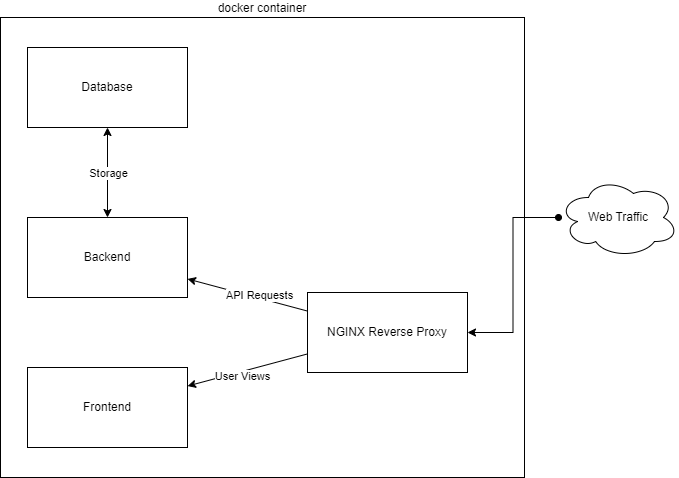
\includegraphics[scale=0.7]{Design/SystDesign/stack-graph.png}
    \caption{A component graph diagram for the application stack}
    \label{fig:my_label}
\end{figure}

At the core of the platform is the backend, which is built with Django and PostgreSQL. This is connected to the frontend, built with Next.js and is served by an NGINX web server. This allows for a smooth and efficient experience for both the developers and in production.

\noindent The stack can be deployed as a Docker container making it more scalable, as more worker nodes can be added dynamically as load increases. 

\subsection{Connection Between Requirements and Design} \label{SecConnection}

\wss{The intention of this section is to document decisions that are made
  ``between'' the requirements and the design.  To satisfy some requirements,
  design decisions need to be made.  Rather than make these decisions implicit,
  they are explicitly recorded here.  For instance, if a program has security
  requirements, a specific design decision may be made to satisfy those
  requirements with a password.}

  % Ethan - make it more abstract

\section{System Variables}

\subsection{Monitored Variables}
\begin{itemize}
    \item Customer location: The location of the customer is monitored to provide relevant shop suggestions based on proximity.
    \item Shop availability: The availability of shops is monitored to ensure customers can book appointments only when shops have open slots.
    \item Customer quote requests: The platform monitors incoming quote requests from customers to facilitate timely responses from shops.
    \item Employee schedules: Employee schedules are monitored to ensure accurate appointment booking and prevent overbooking.
    \item Customer feedback: Customer feedback and ratings are monitored to maintain a high-quality service experience.
\end{itemize}

\subsection{Controlled Variables}
\begin{itemize}
    \item Shop capacity: The platform controls the maximum number of appointments a shop can handle at a given time.
    \item Shop services: The platform allows shop owners to define and control the services they offer.
    \item Appointment scheduling: The platform controls the scheduling of appointments based on shop and employee availability.
    \item Employee access: The platform controls employee access to specific shop tools and information.
    \item Customer notifications: The platform controls the notifications sent to customers regarding appointment status, quotes, and other relevant information.
\end{itemize}

\subsection{Constants Variables}
\begin{itemize}
    \item Shop licensing: The platform ensures that only licensed shops are allowed to create a digital storefront and offer services.
    \item Service categories: The platform maintains a constant list of service categories that shops can choose from when defining their services.
    \item User roles: The platform has predefined user roles (customer, shop owner, employee) with specific access and functionalities.
    \item Appointment duration: The platform maintains a constant appointment duration for each service type, which can be customized by the shop owner if needed.
\end{itemize}

\section{User Interfaces}

% Frontend
%   Auth - Kai
%   Profile
    % Customer - Ethan
        % Vehicles
    % Shop Owner - Ethan
    % Employee - Ethan
%   ShopLookup - Collin
%   Quotes - Alyssa
%   QuoteRequest - Alyssa
%   Homepages - Ethan
%   Shop - Chris
%       Services
%   Apppointment - Harsh
%   Workorders - Harsh

\wss{Design of user interface for software and hardware.  Attach an appendix if
needed. Drawings, Sketches, Figma}

\subsection{Authentication UI}
UIs relating to authentication, registration, and password recovery are shown in Figure \ref{fig:authUI}. 

\subsection{Customer QuoteRequest UI}
UIs relating to customer quote request creation, modification, viewing are shown starting at figure \ref{fig:quoteRequestUI1}.

\subsection{Diagrams of Shop Quotes}
UIs relating to shop quote approval, viewing, and modification are shown starting at figure \ref{fig:quoteUI1}.

\subsection{Diagrams of Shop Creation}
UIs relating to shop creation, which is only displayed when a Shop Owner first logs in, is shown in Figure \ref{fig:ShopCreateUI}.

\subsection{Customer Shop Lookup UI}
UIs relating to the customer shop lookup. Name and address of all shops are displayed, and users can click a certain shop to view more details (e.g. shop services). Shown in Figure \ref{fig:shopLookupUI}.

\section{Design of Hardware}

N/A

\section{Design of Electrical Components}

N/A

\section{Design of Communication Protocols}

N/A

\section{Timeline}
\noindent \textbf{Document revision 0}
\begin{itemize}
    \item Deadline: February 10th
    \item To be completed by: All team members
\end{itemize}

\noindent \textbf{Document revision 1}
\begin{itemize}
    \item Deadline: April 5th
    \item To be completed by: All team members
\end{itemize}

\noindent \textbf{Completion of implementing frontend specific modules}
\begin{itemize}
    \item Deadline: February 7th
    \item To be completed by: All team members working on their own respective modules.
    \item Auth, Profile: Kai
    \item Customer, ShopOwner, Homepage: Ethan
    \item ShopLookup: Collin
    \item Quotes, QuoteRequest: Alyssa
    \item Shop, Services: Chris
    \item Appointment, WorkOrders: Harsh
\end{itemize}

\noindent \textbf{Completion of implementing backend specific modules}
\begin{itemize}
    \item Deadline: February 7th
    \item To be completed by: All team members working on their own respective modules.
    \item Auth, Profile: Kai
    \item Customer, ShopOwner, Homepage: Ethan
    \item ShopLookup: Collin
    \item Quotes, QuoteRequest: Alyssa
    \item Shop, Services: Chris
    \item Appointment, WorkOrders: Harsh
\end{itemize}

\noindent \textbf{Initial testing for revision 0 - ensure all components function and are presentable}
\begin{itemize}
    \item Deadline: February 12th
    \item To be completed by: All team members working on their own respective modules
    \item Auth, Profile: Kai
    \item Customer, ShopOwner, Homepage: Ethan
    \item ShopLookup: Collin
    \item Quotes, QuoteRequest: Alyssa
    \item Shop, Services: Chris
    \item Appointment, WorkOrders: Harsh
\end{itemize}

\noindent \textbf{Code Refactoring}
\begin{itemize}
    \item Deadline: March 20th - March 31st
    \item To be completed by: Alyssa, Ethan, Chris, Collin
\end{itemize}

\noindent \textbf{Application Testing}
\begin{itemize}
    \item Deadline: March 20th - March 31st
    \item To be completed by: All team members testing their own respective implementations of the application. Once completed, testing will be conducted on each other's implementations to ensure coverage is sufficient.
\end{itemize}

\noindent \textbf{Application Deployment}
\begin{itemize}
    \item Deadline: March 20th - March 31st
    \item To be completed by: Harsh, Kai
\end{itemize}

\noindent \textbf{Final Feature Implementation Based on MVP, Post-MVP}
\begin{itemize}
    \item Deadline: March 20th - March 31st
    \item To be completed by: All team members for their respective features they are implementing.
    \item Auth, Profile: Kai
    \item Customer, ShopOwner, Homepage: Ethan
    \item ShopLookup: Collin
    \item Quotes, QuoteRequest: Alyssa
    \item Shop, Services: Chris
    \item Appointment, WorkOrders: Harsh
\end{itemize}

\newpage{}

\appendix


\section{Interface}
\subsection{Authentication UI}
\begin{figure}[H]
    \centering
    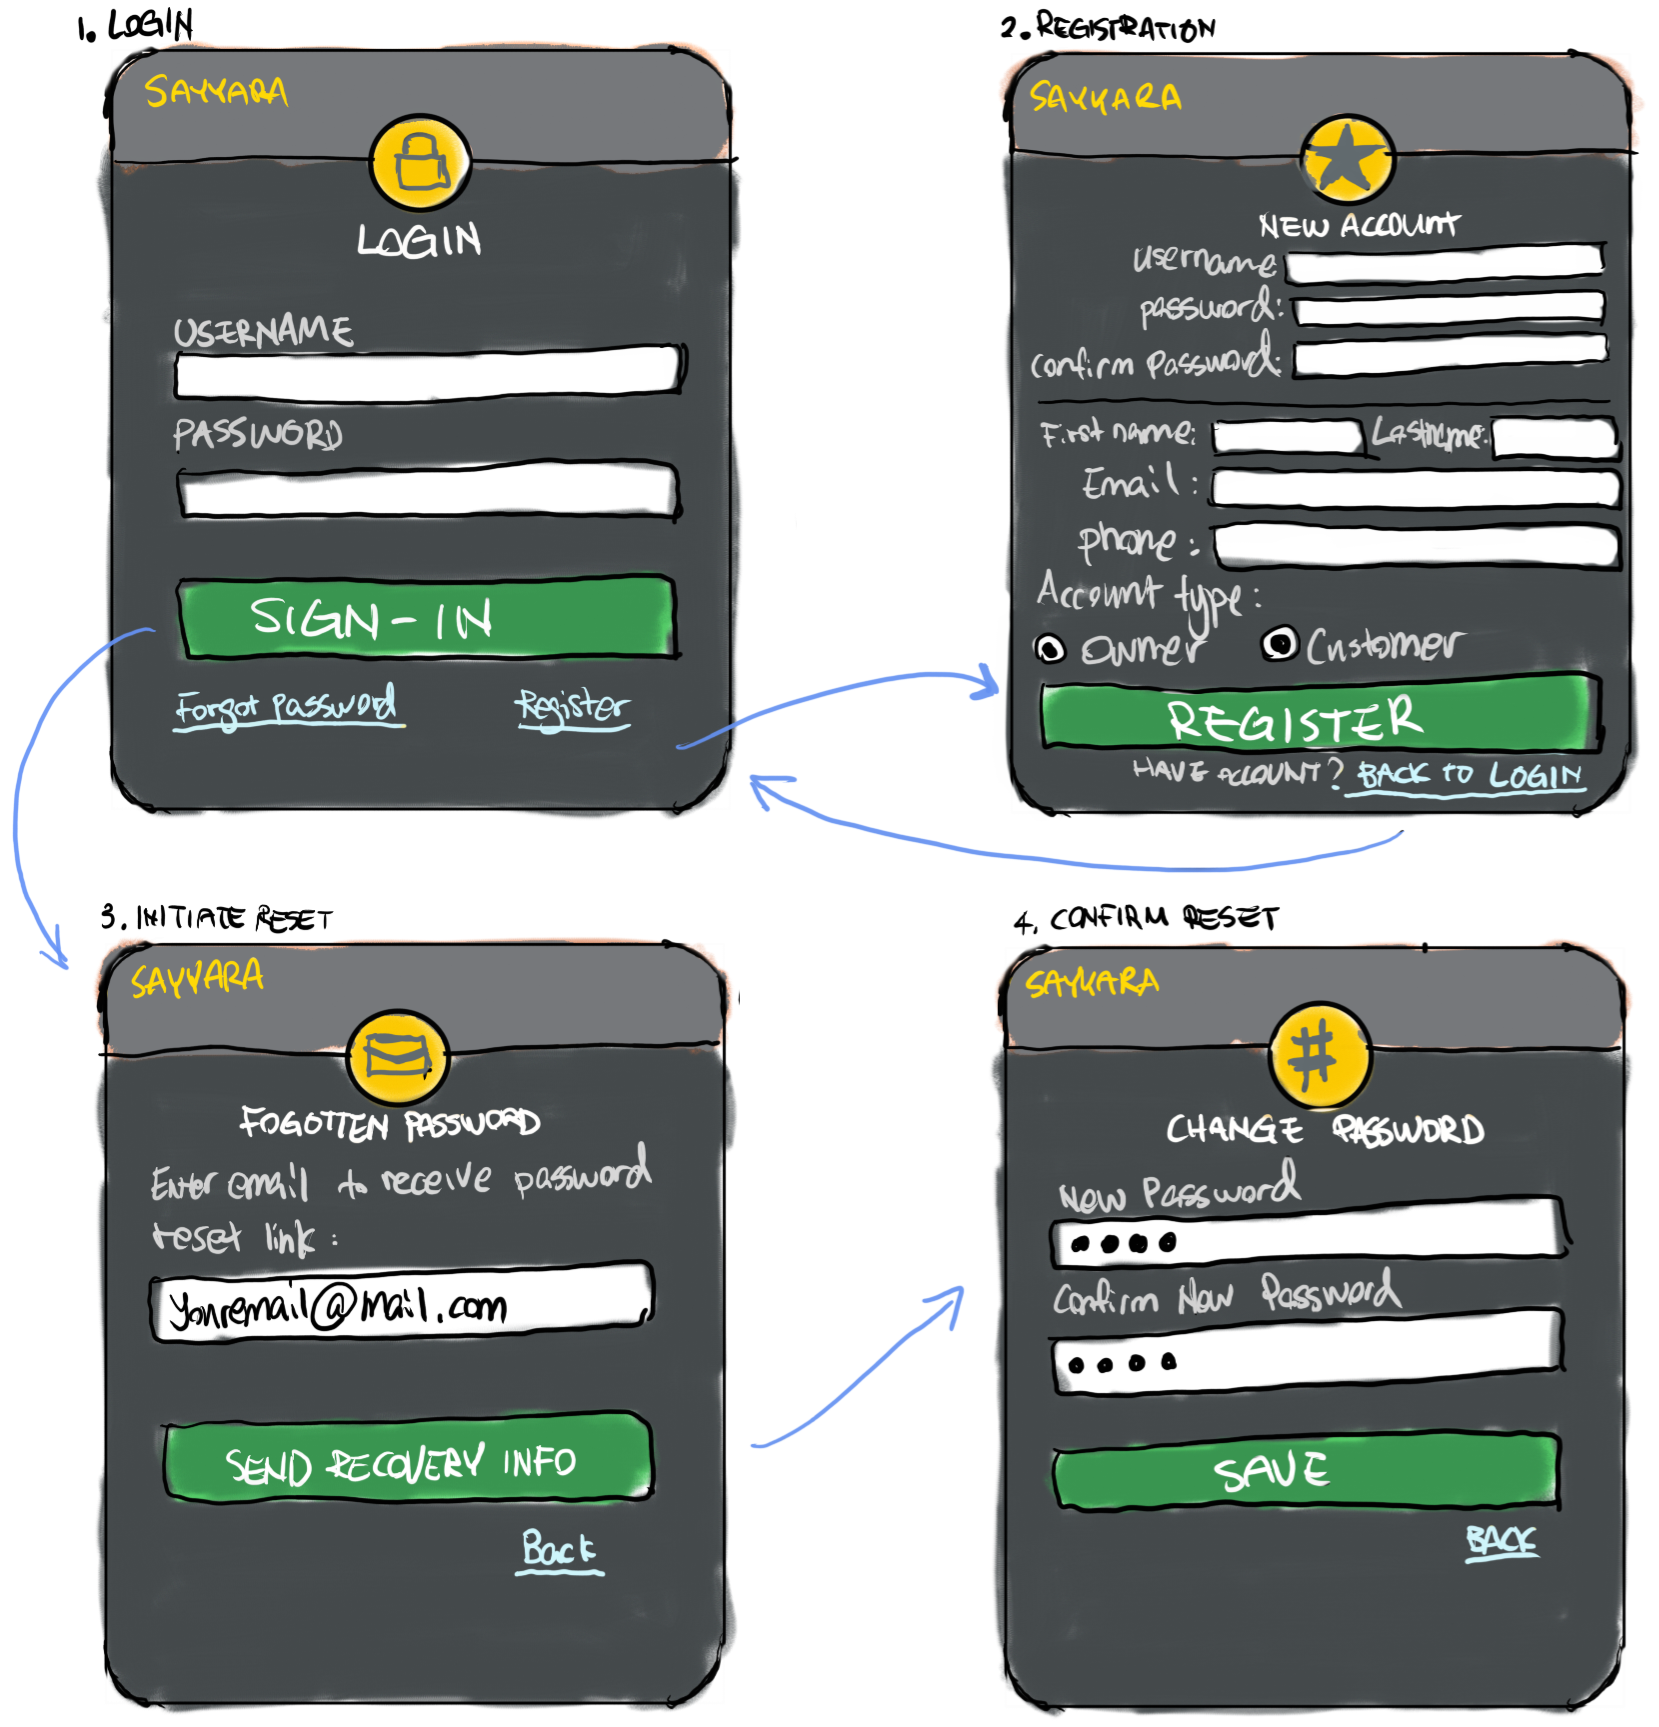
\includegraphics[width=\textwidth]{Design/SystDesign/ui_auth.png}
    \caption{Authentication module includes 4 UI: login, register, initiate password recovery, and confirm password reset. Blue arrows mark the navigation flow between the UIs.}
    \label{fig:authUI}
\end{figure}

\subsection{Customer QuoteRequest UI}
\begin{figure}[H]
    \centering
    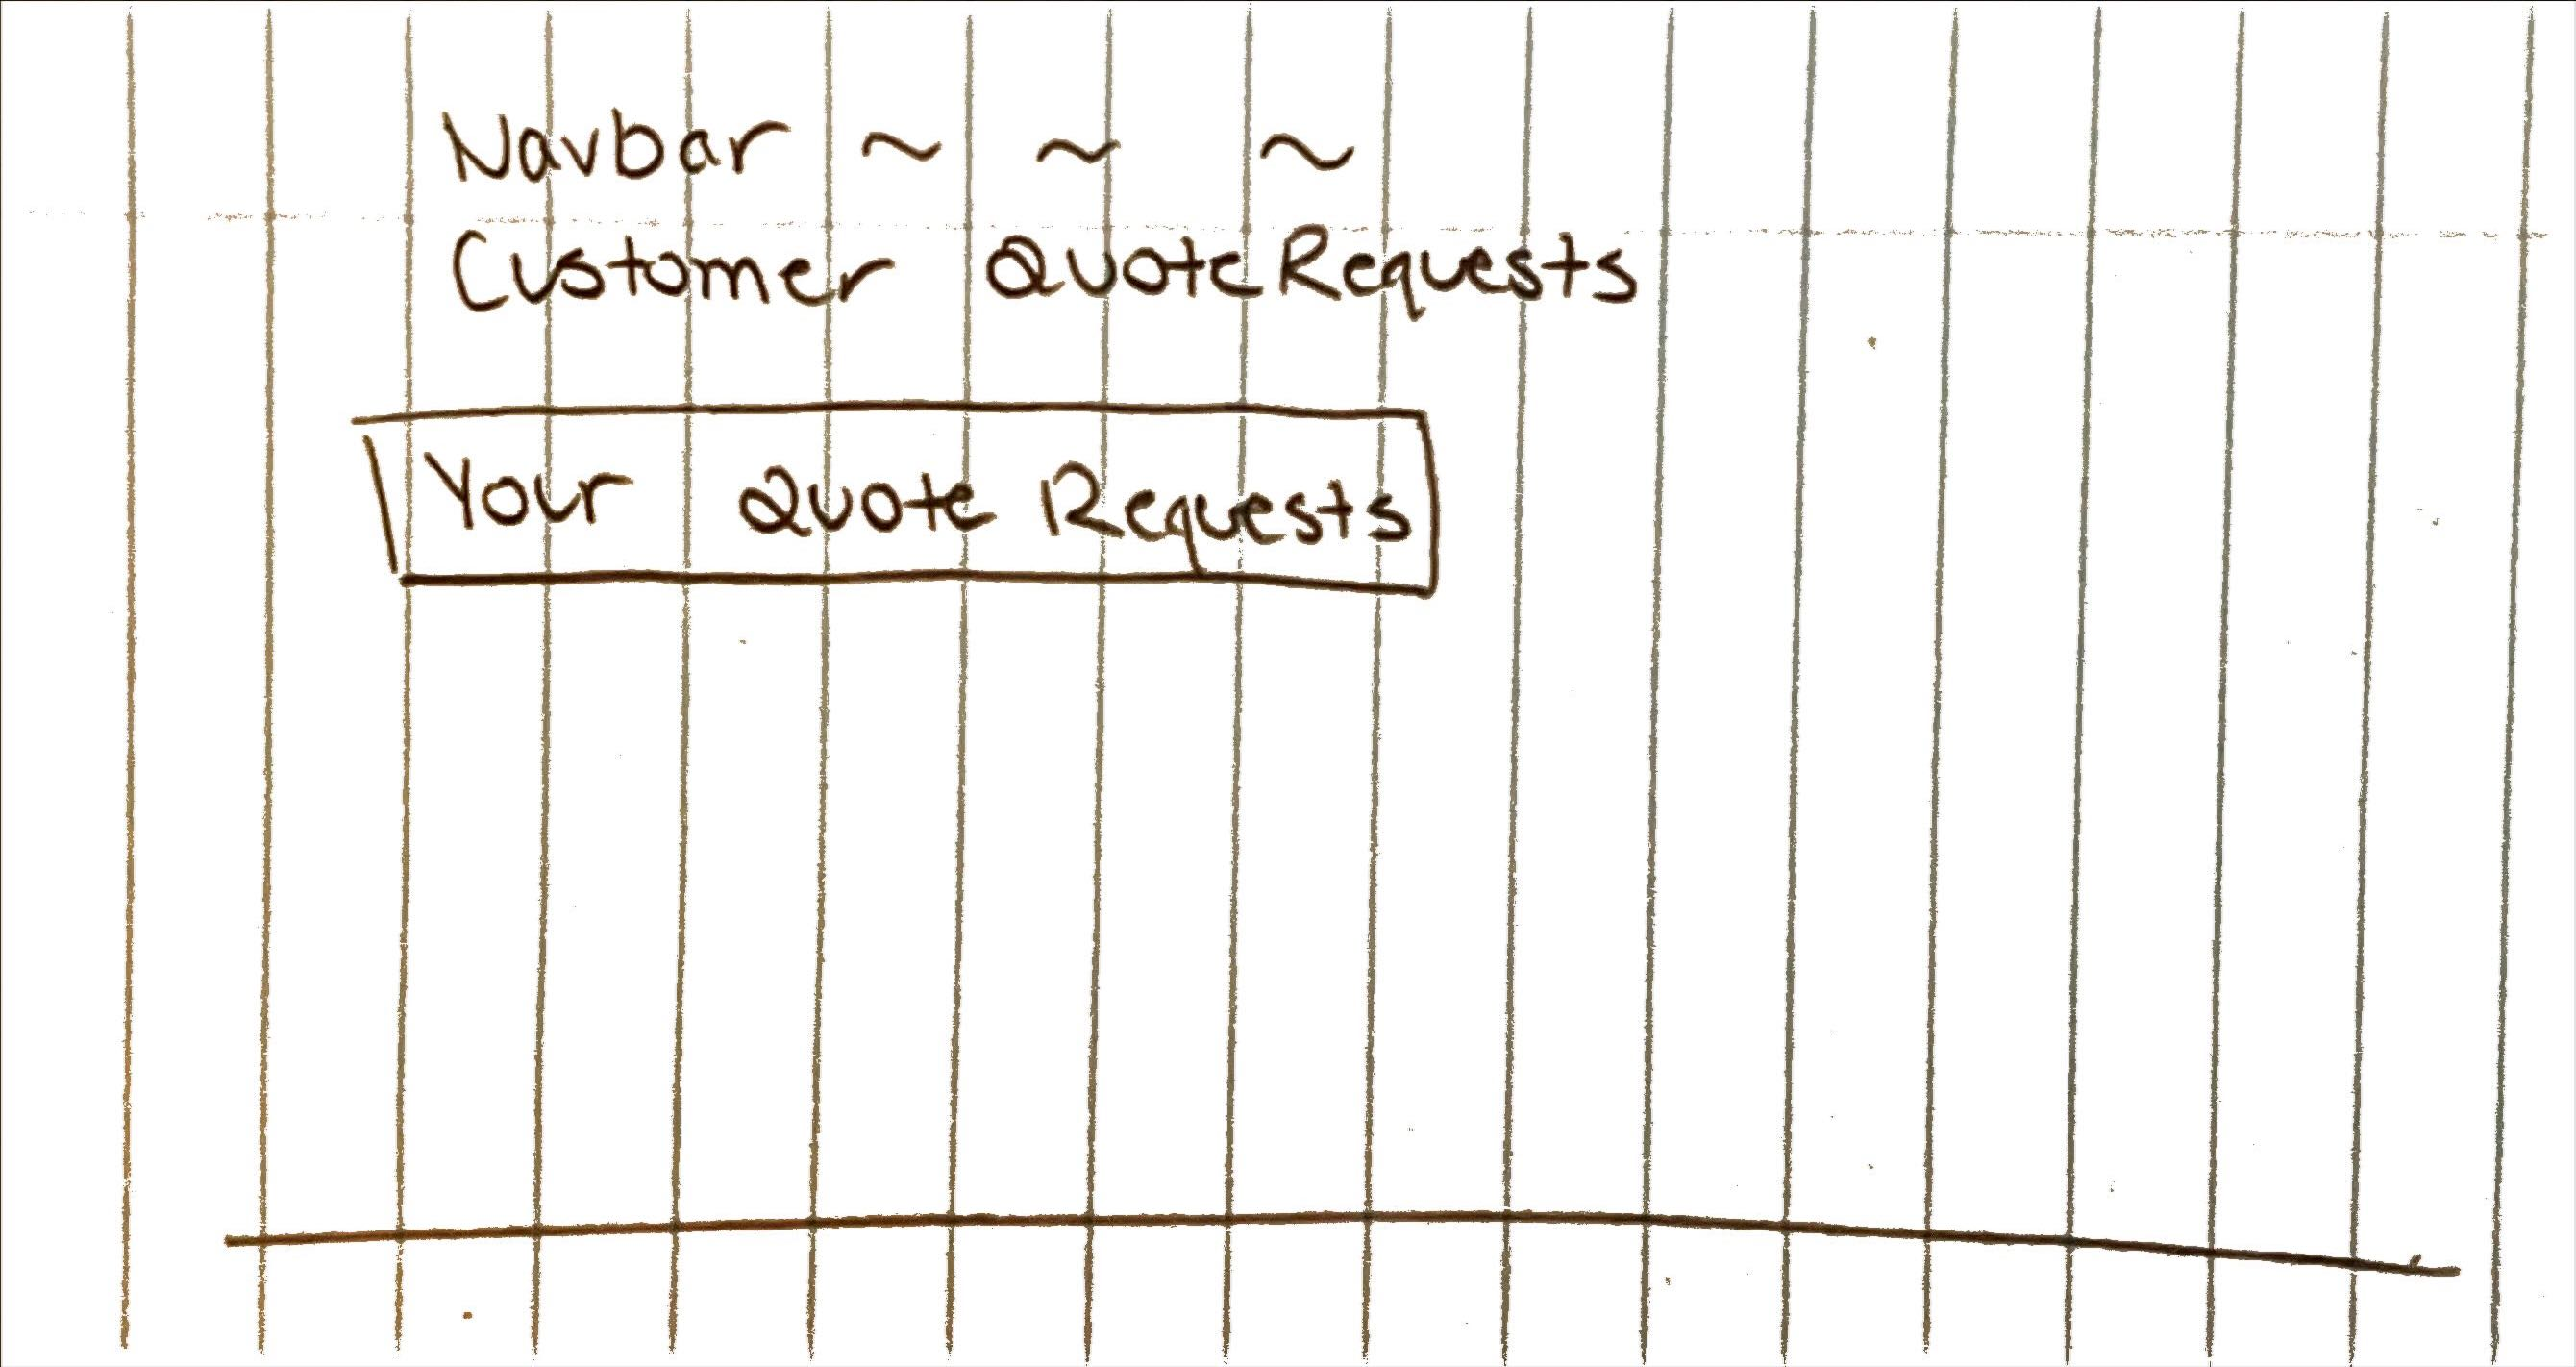
\includegraphics[width=\textwidth]{Design/SystDesign/Quotes/QuoteRequest1.png}
    \caption{Customer quote request UI with an option for the customer to display their currently created quote requests.}
    \label{fig:quoteRequestUI1}
\end{figure}

\begin{figure}[H]
    \centering
    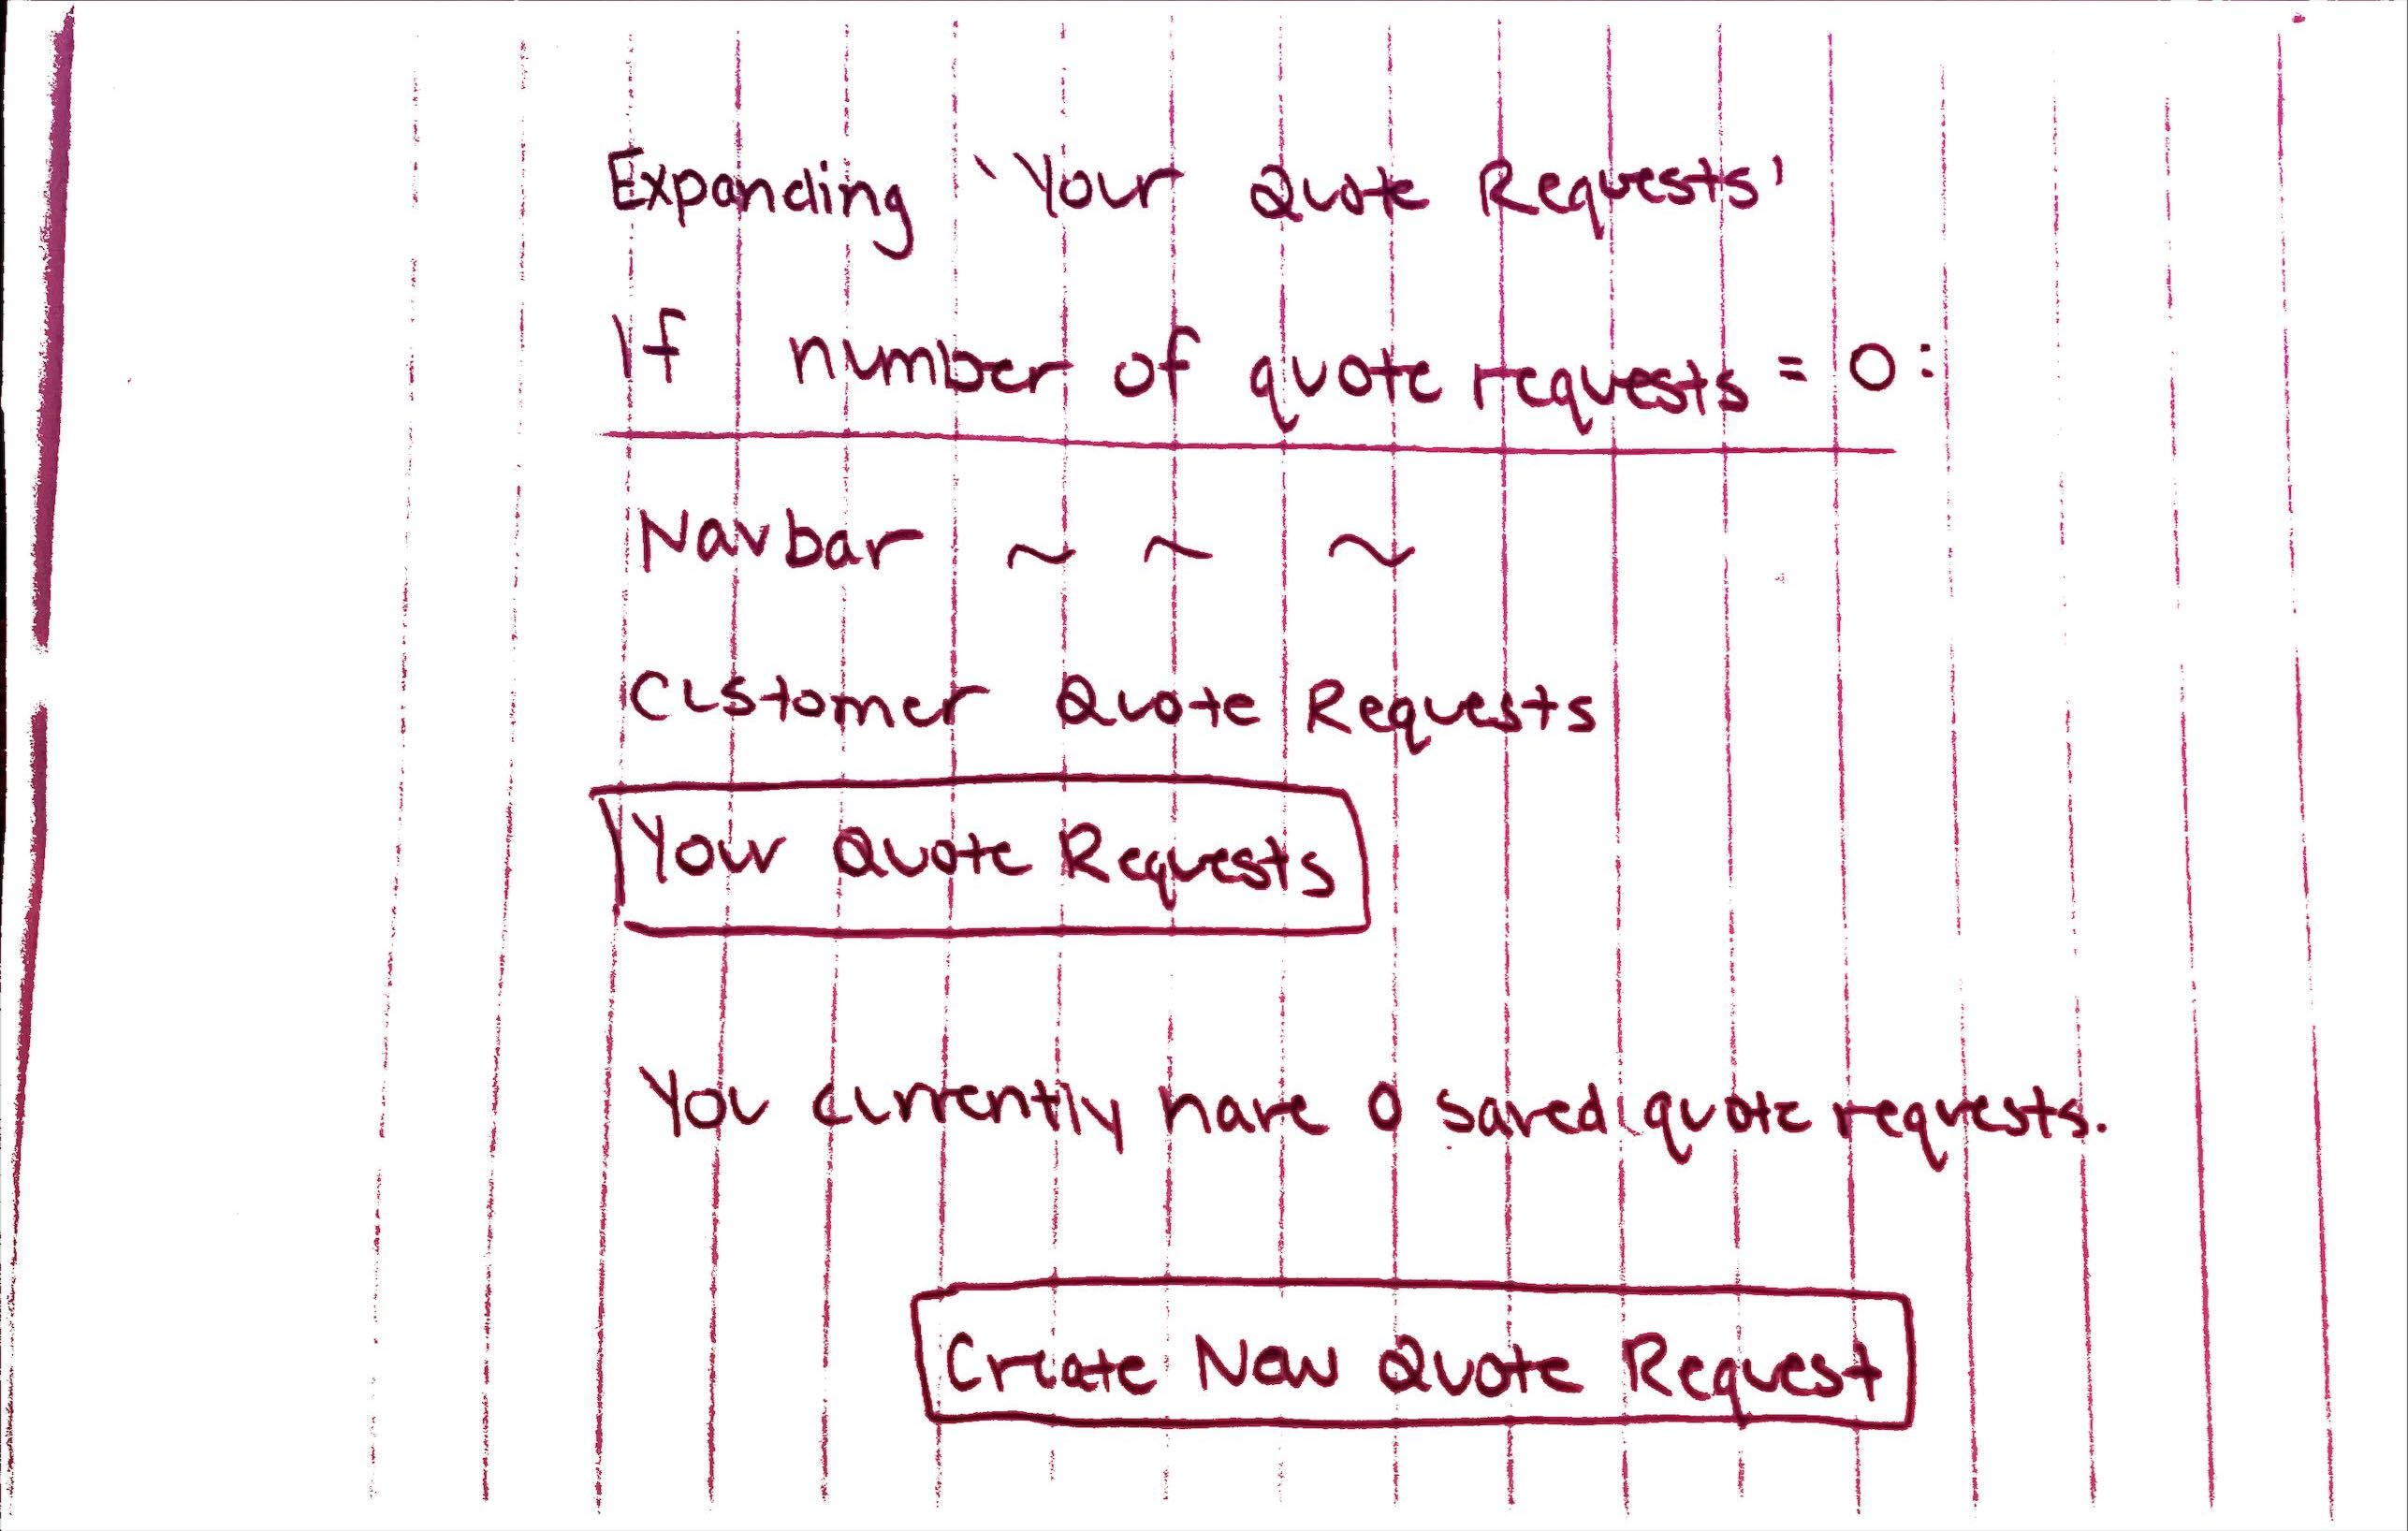
\includegraphics[width=\textwidth]{Design/SystDesign/Quotes/QuoteRequest2.png}
    \caption{Customer quote request UI when the user selects 'Your Quote Requests' and there are no saved quote requests. The user has the option to create a new quote request.}
    \label{fig:quoteRequestUI2}
\end{figure}

\begin{figure}[H]
    \centering
    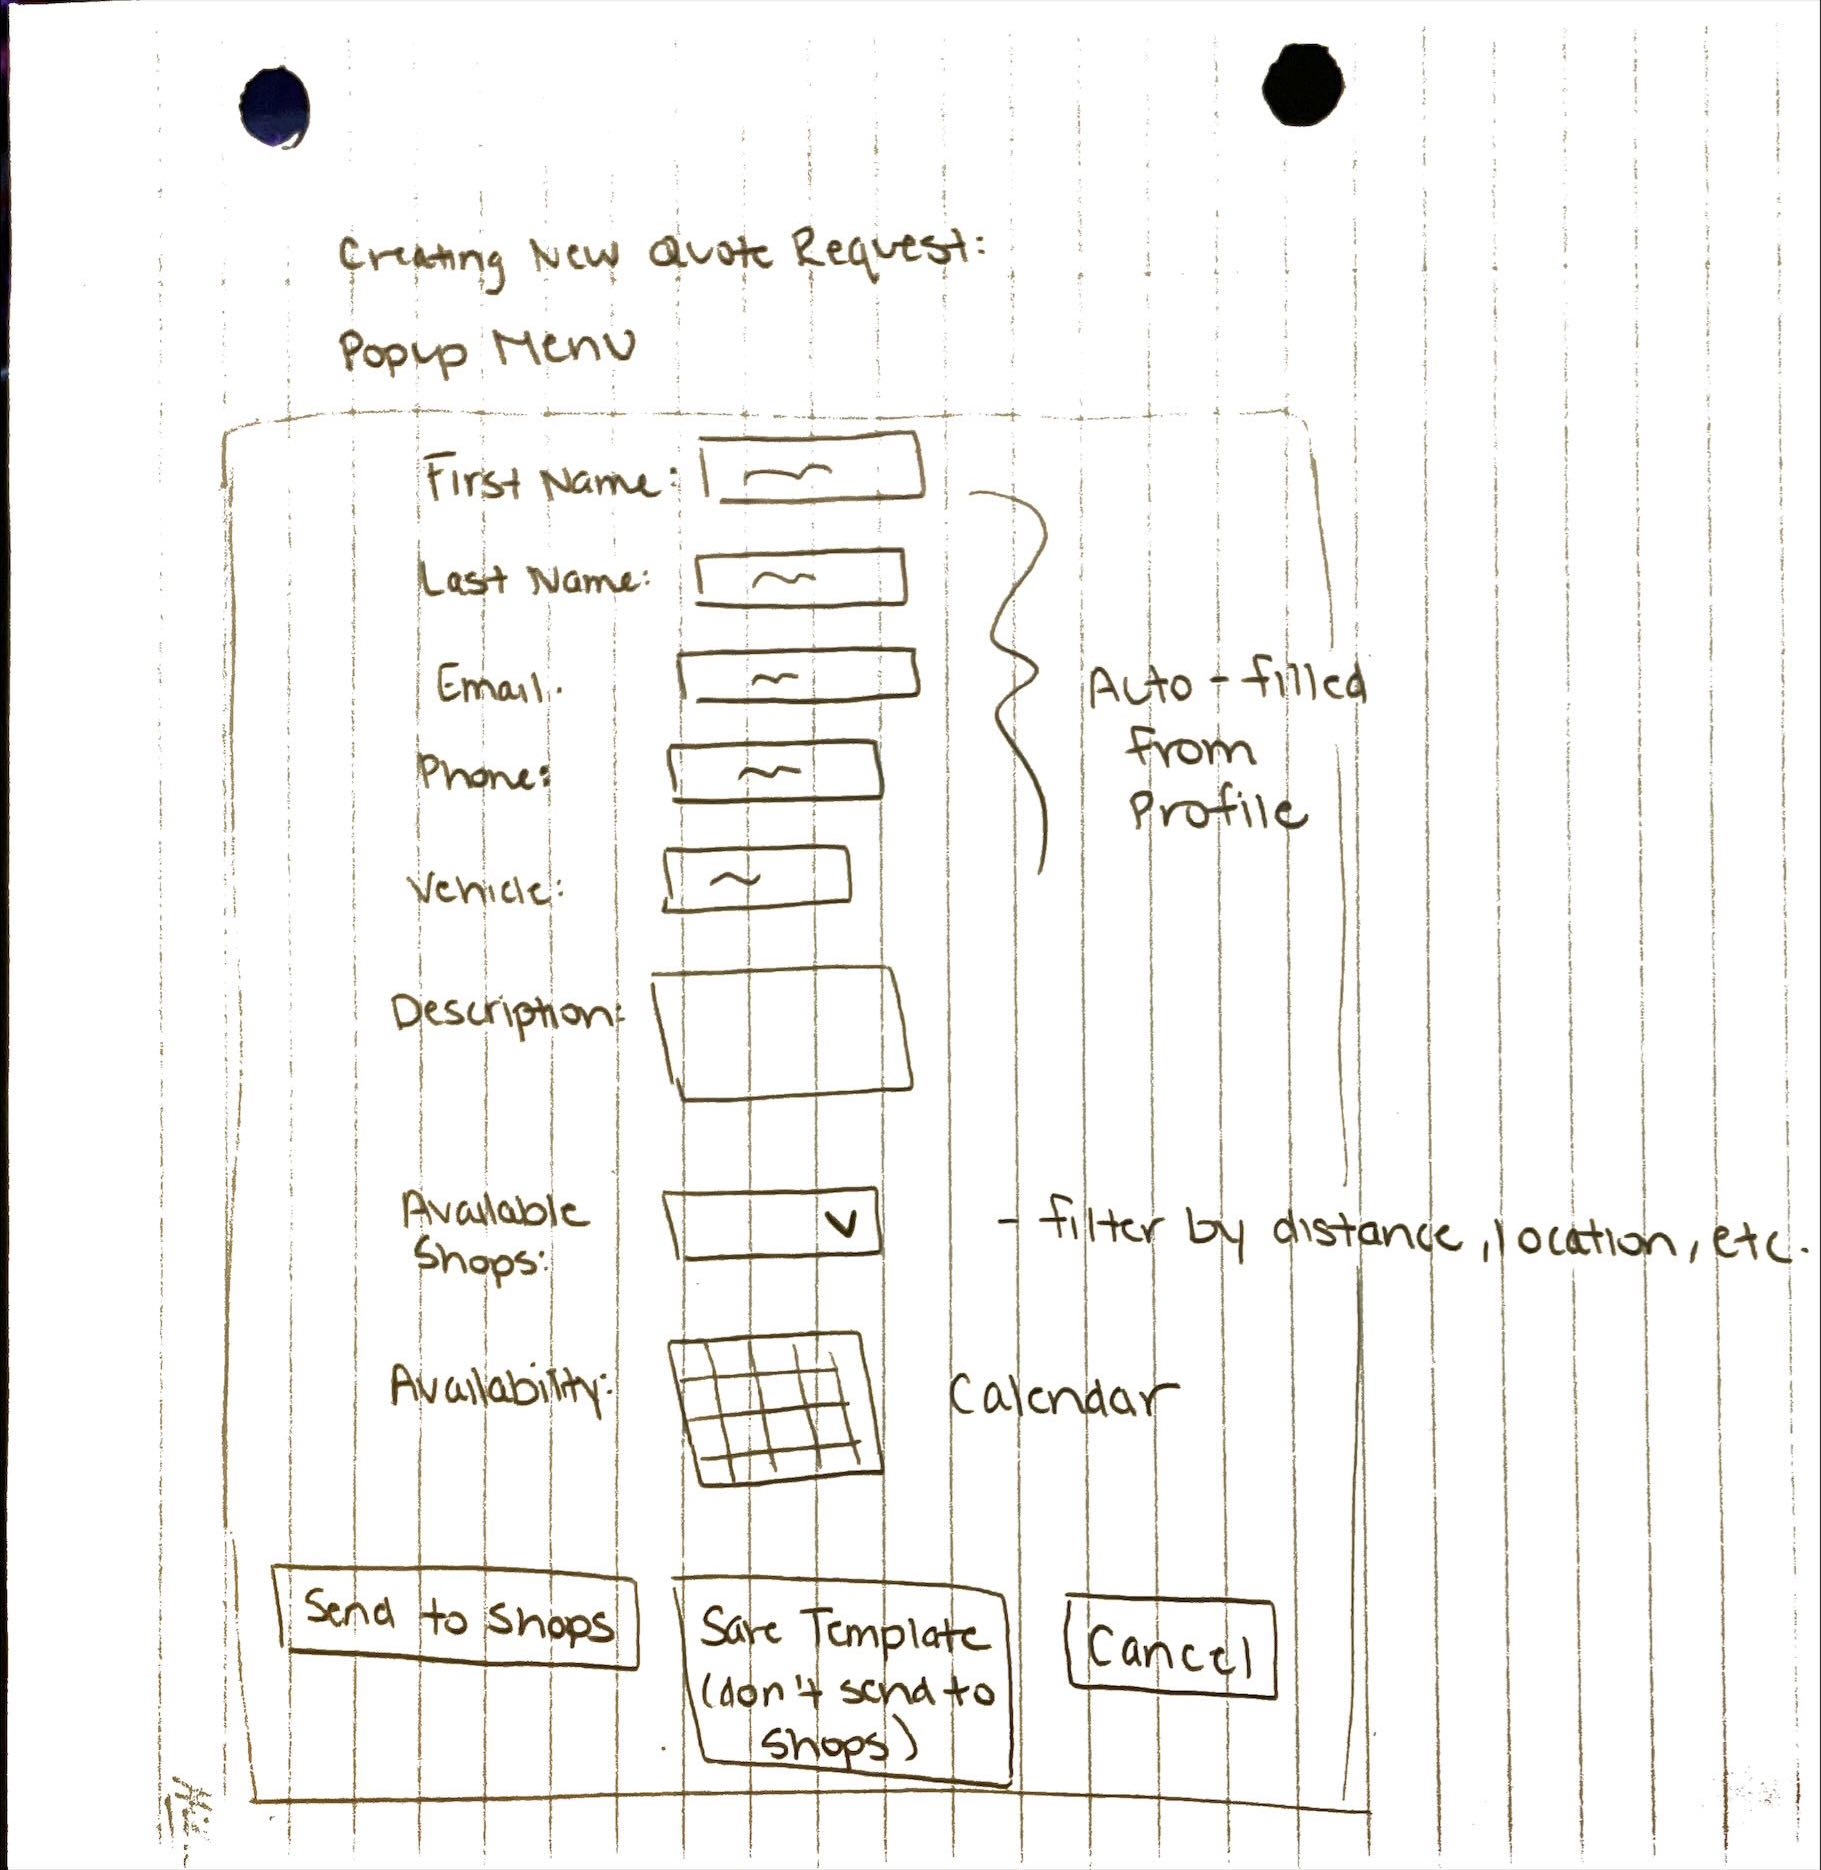
\includegraphics[width=\textwidth]{Design/SystDesign/Quotes/QuoteRequest3.png}
    \caption{Customer quote request UI when the user selects 'Create New Quote Request'. A popup menu will display with some information populated from their profile. They have the option to send this to multiple shops from a dropdown style searchable list. The user can then send this information to selected shops, or save the template for later if they decide against sending.}
    \label{fig:quoteRequestUI3}
\end{figure}

\begin{figure}[H]
    \centering
    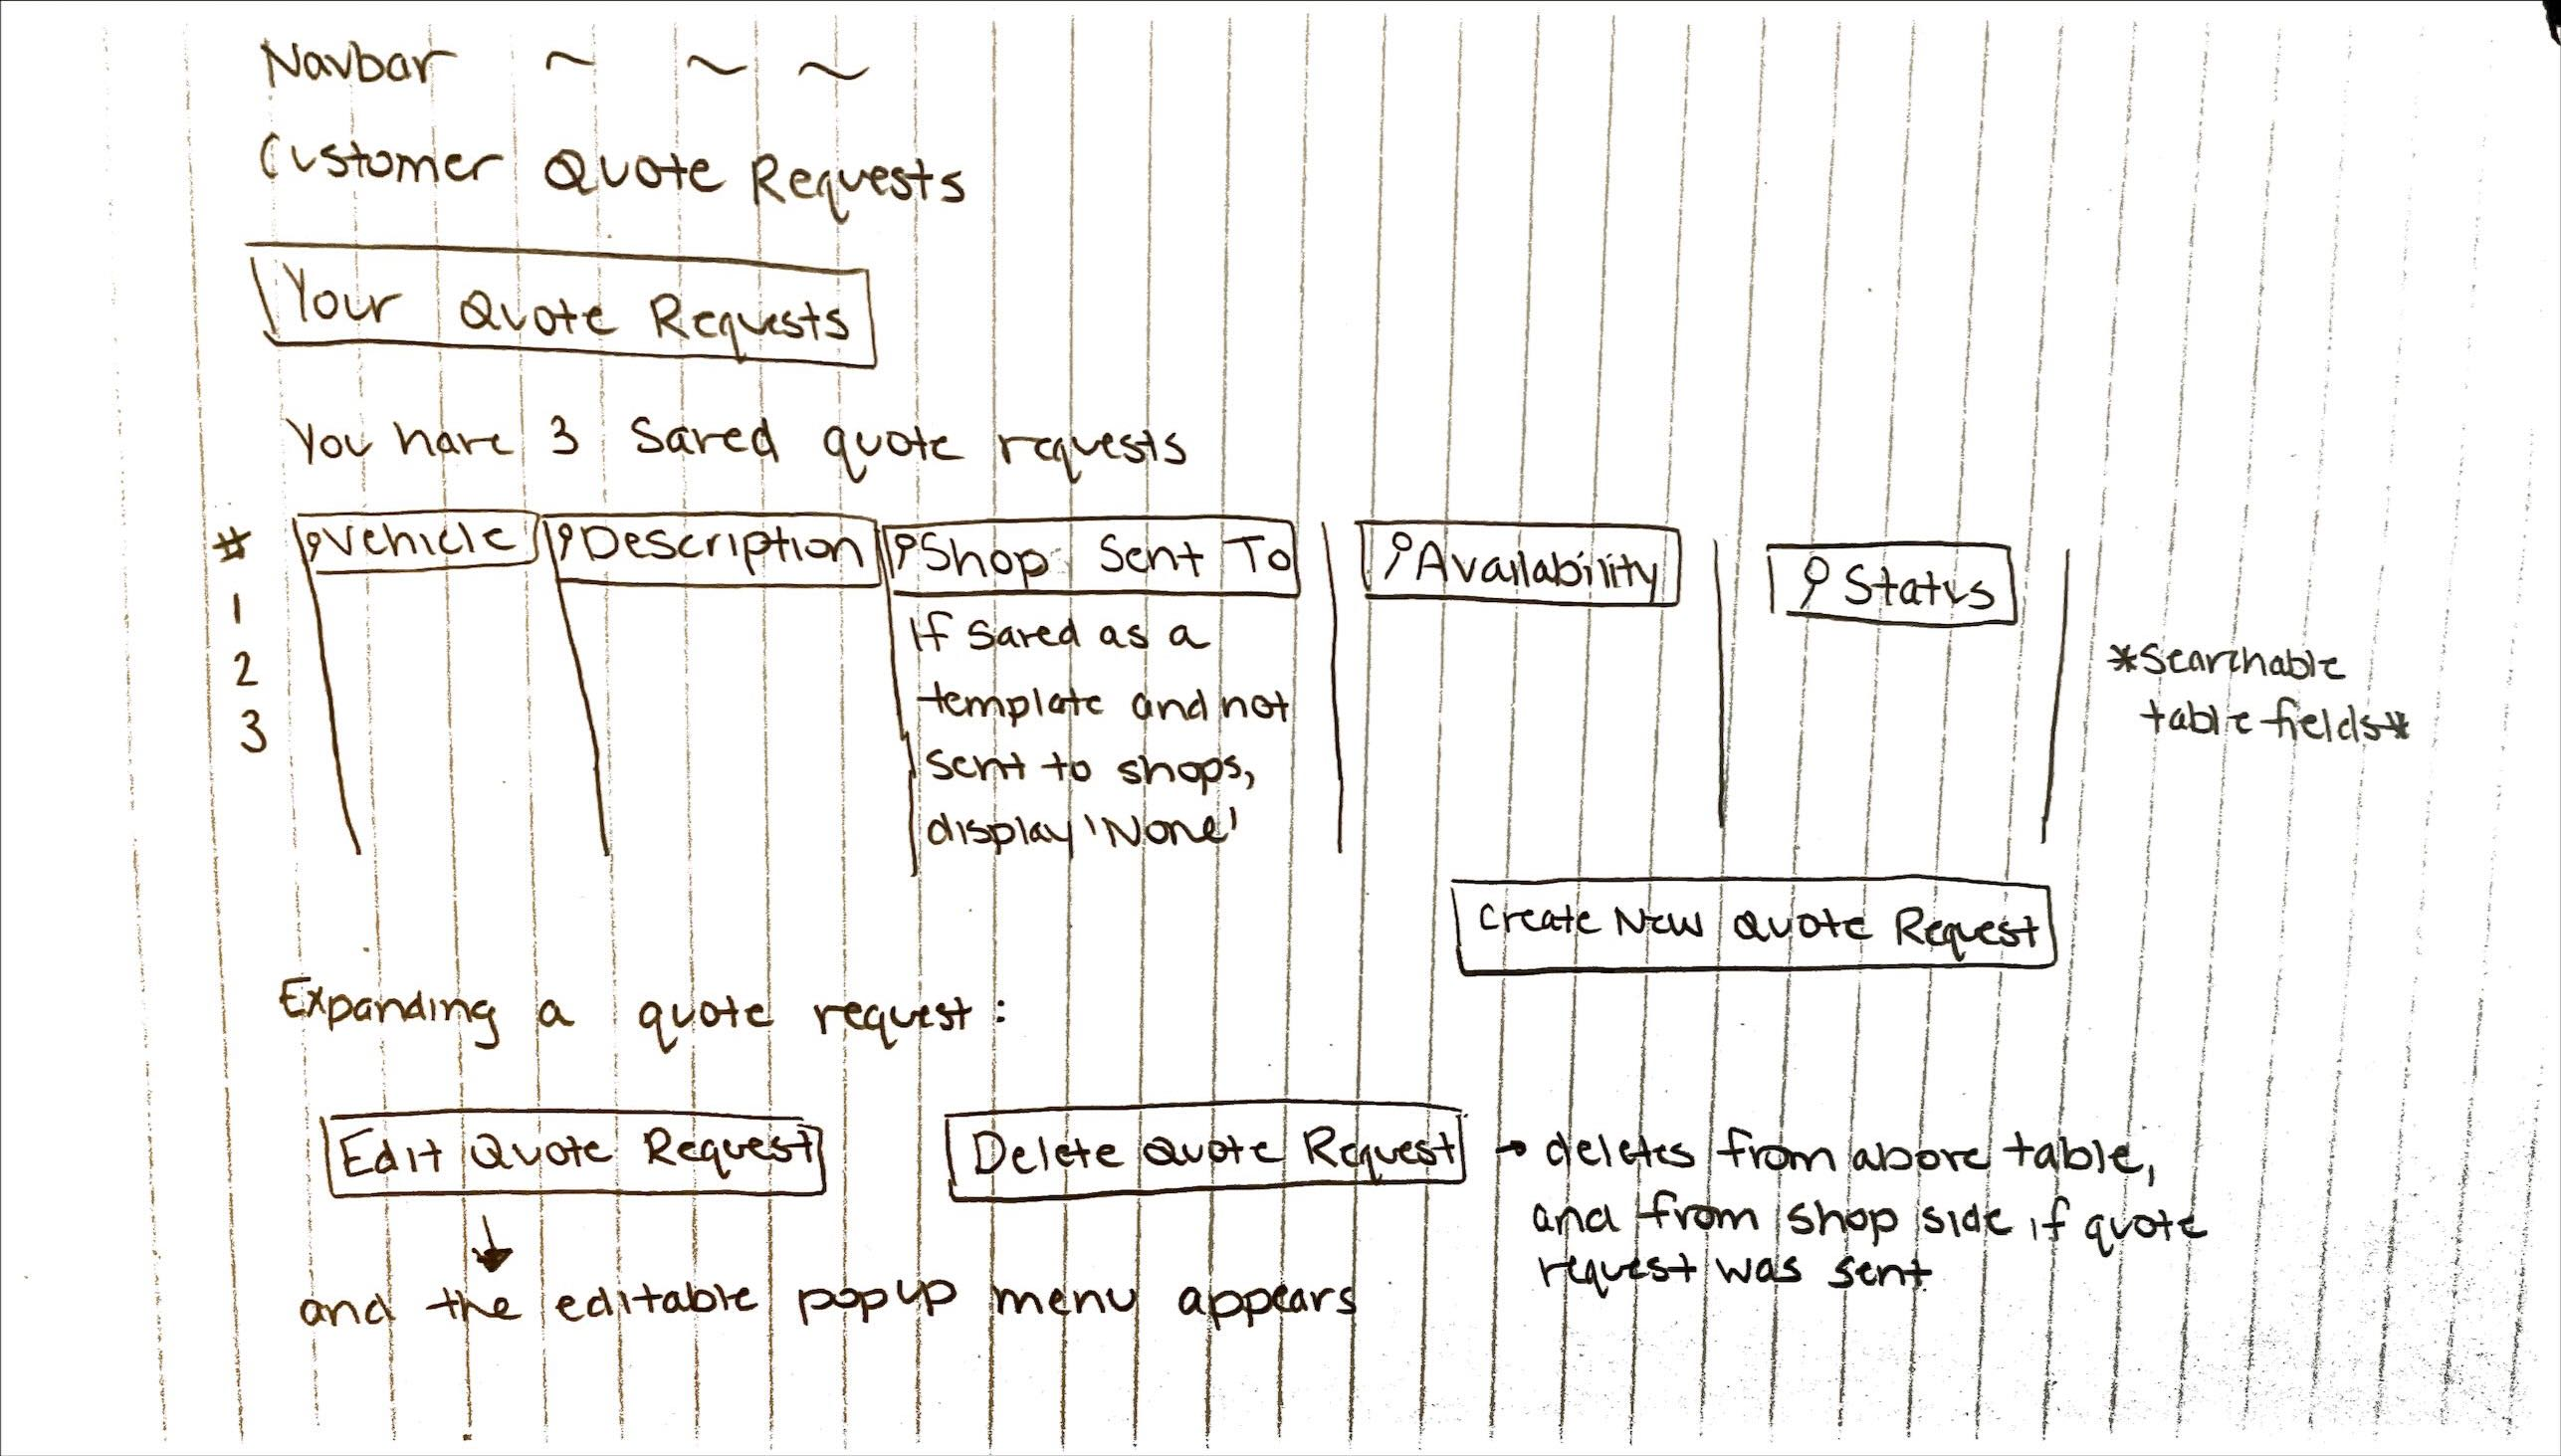
\includegraphics[width=\textwidth]{Design/SystDesign/Quotes/QuoteRequest4.png}
    \caption{Customer quote request UI with save quote request templates displayed for the user when they select 'Your Quote Requests'. If they choose to expand a quote request, they will have the option to edit or delete. For editing, a popup menu similar to \ref{fig:quoteRequestUI3} is displayed. The table of quote requests is also searchable by field.}
    \label{fig:quoteRequestUI4}
\end{figure}


\subsection{Shop Quotes UI}
\begin{figure}[H]
    \centering
    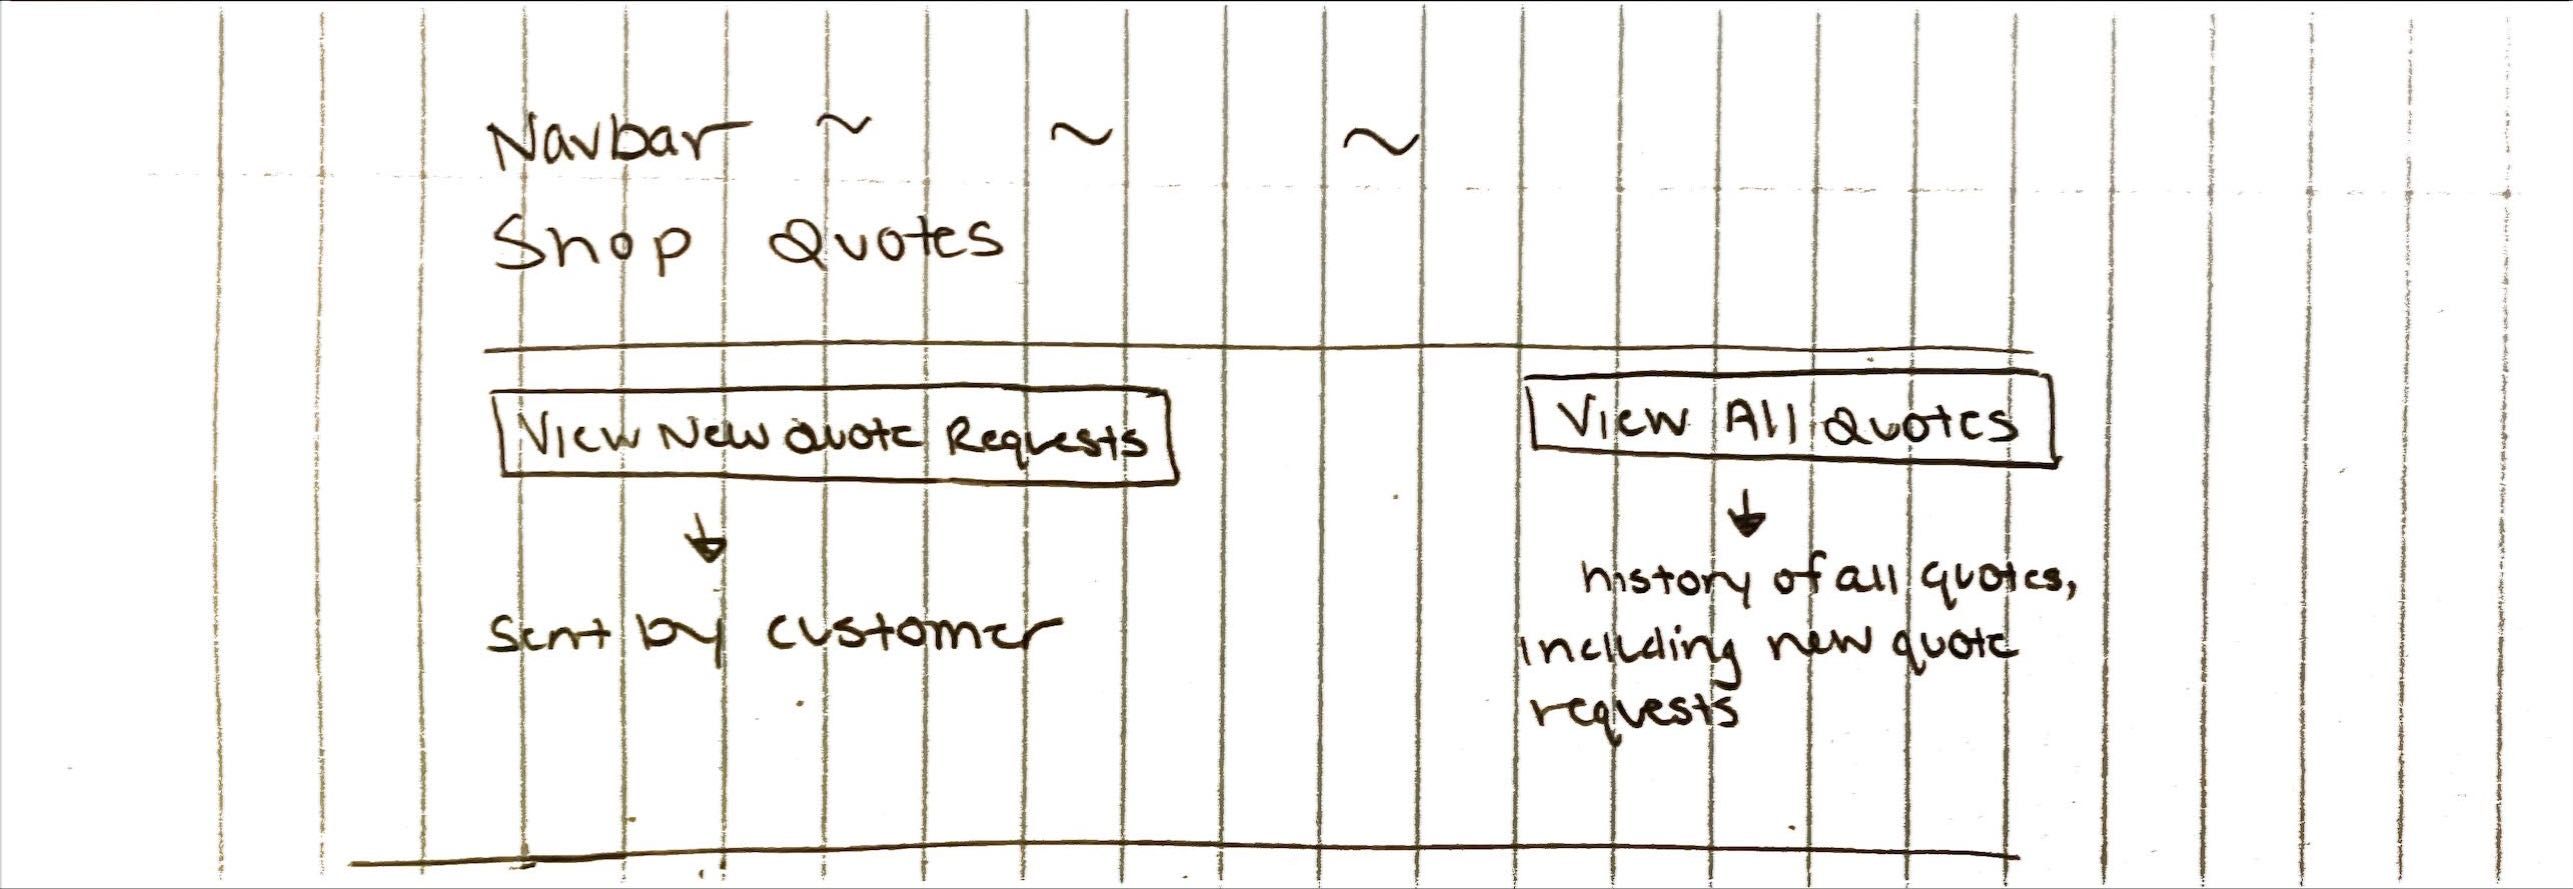
\includegraphics[width=\textwidth]{Design/SystDesign/Quotes/Quote1.png}
    \caption{Shop quote UI with options to 'View New Quote Requests' that were sent by customers to this specific shop, or to 'View All Quotes' to display the history of all quotes, including new quote requests that have yet to be viewed by the shop.}
    \label{fig:quoteUI1}
\end{figure}

\begin{figure}[H]
    \centering
    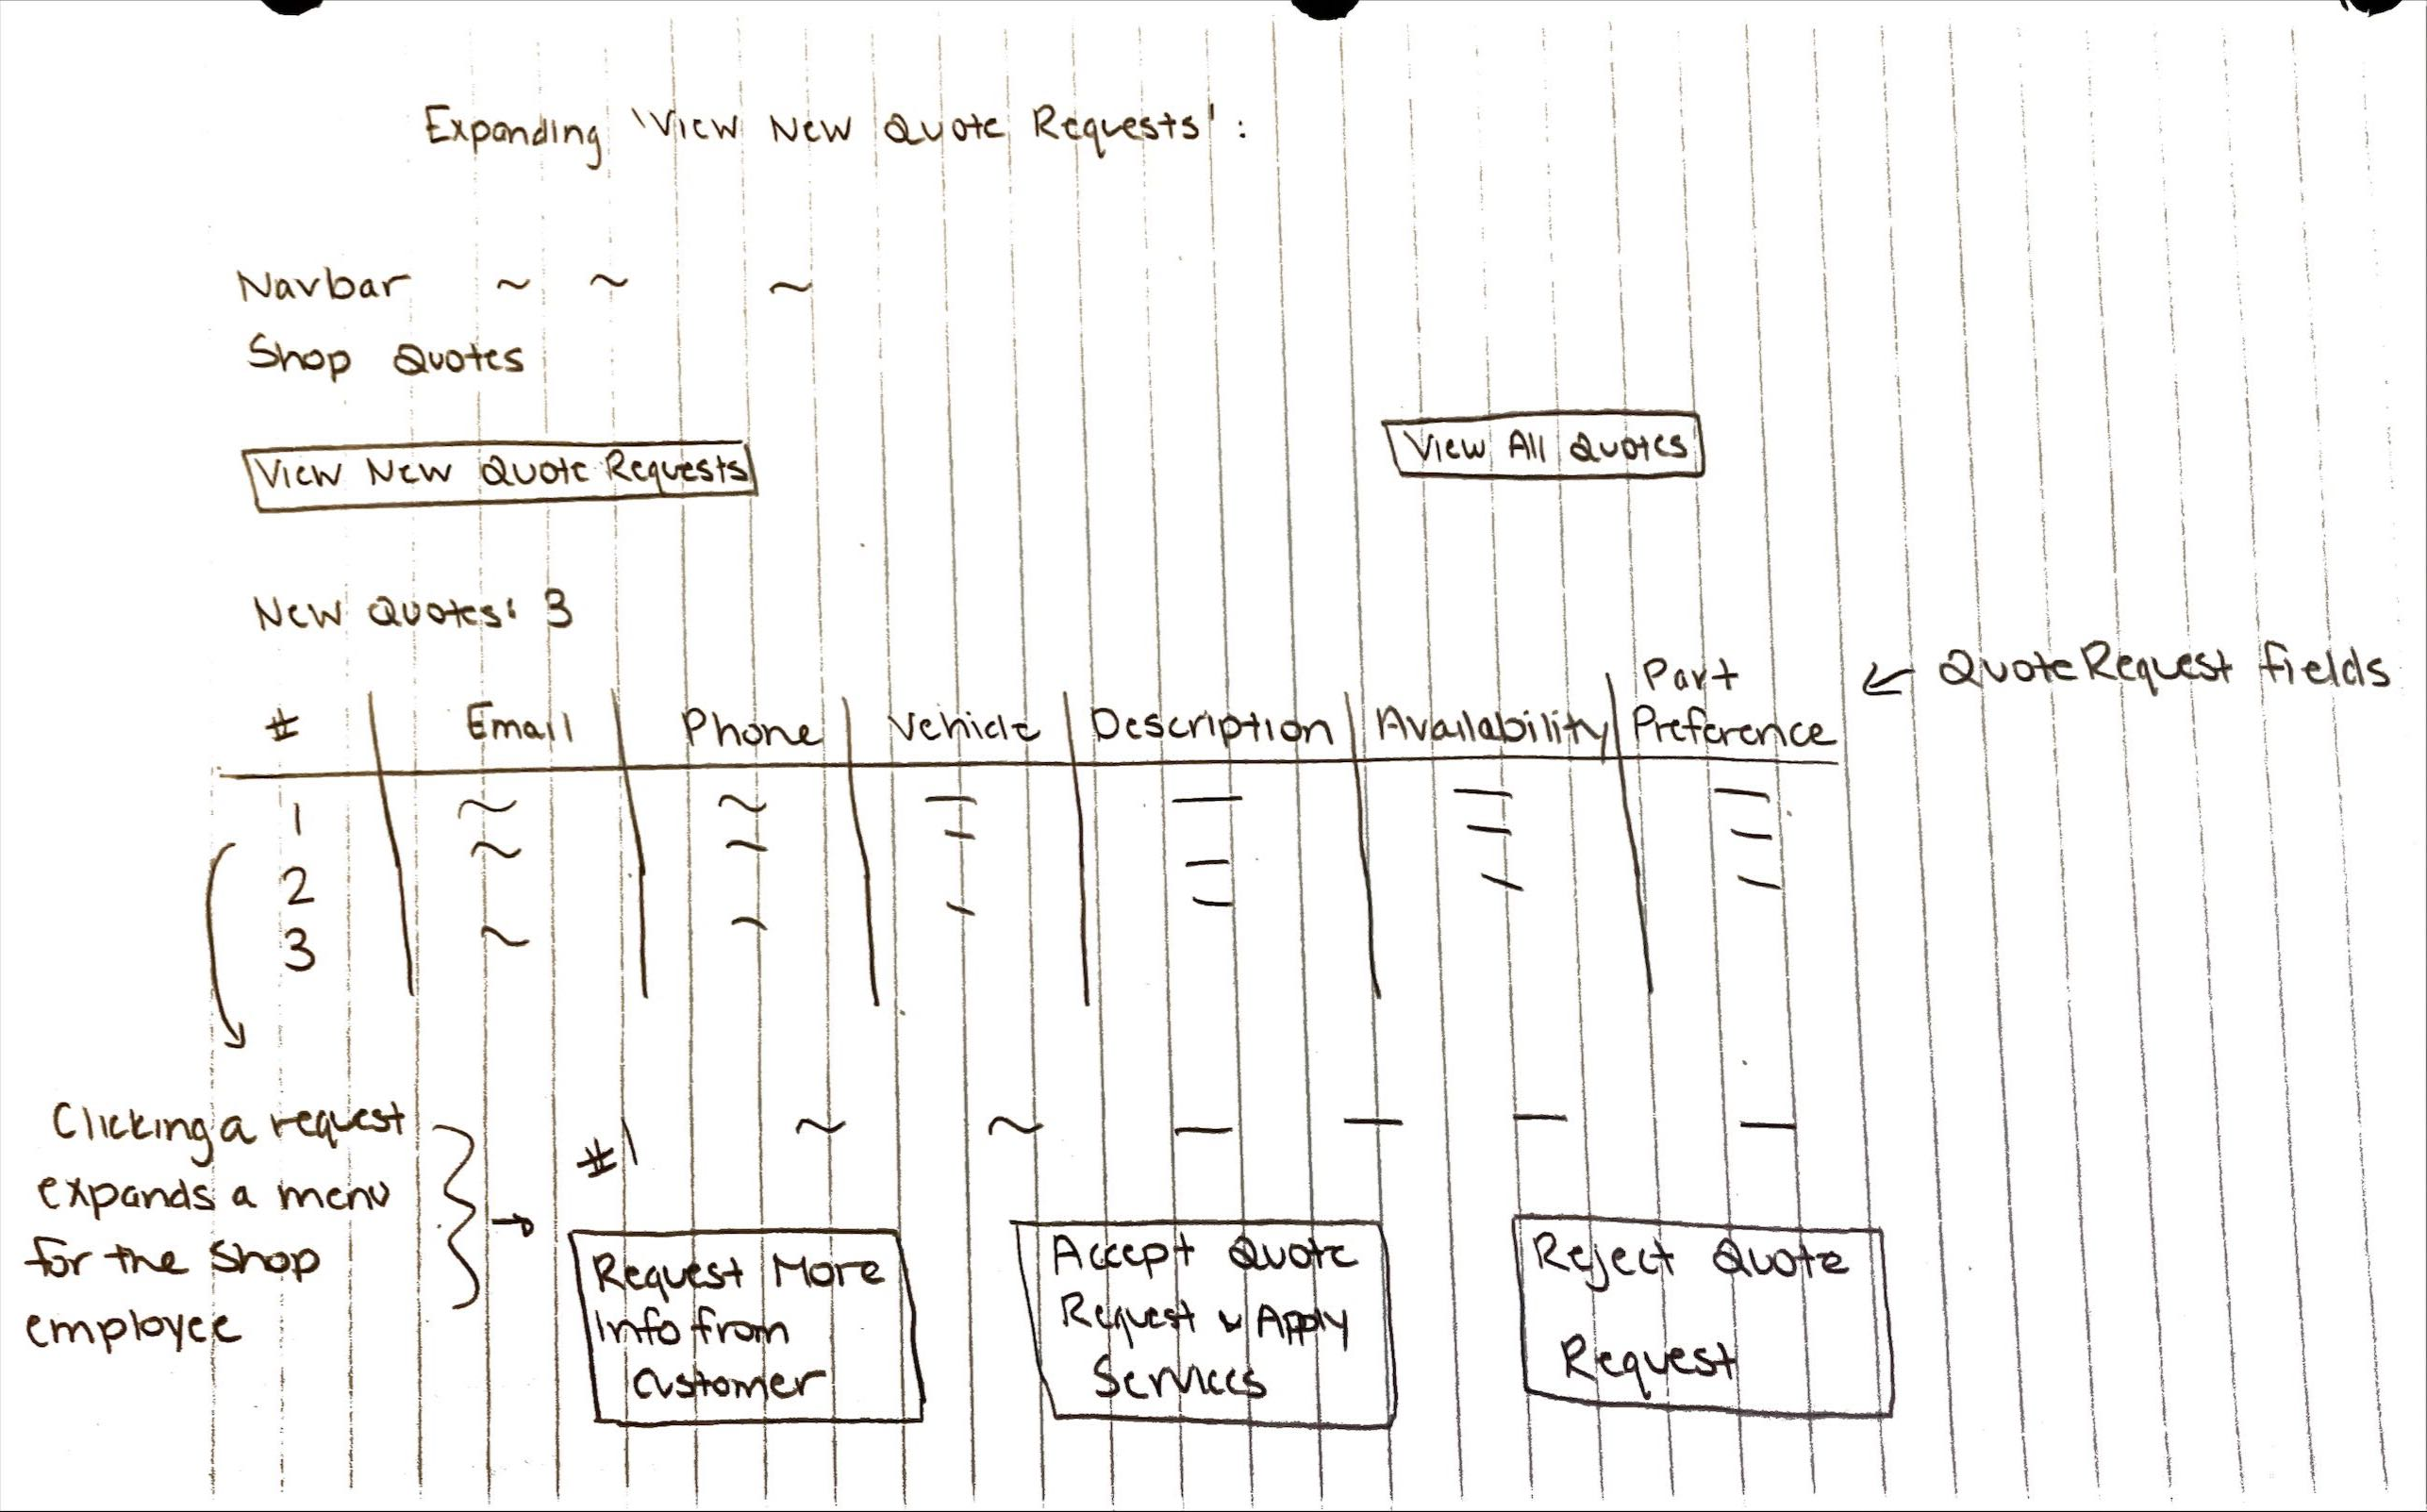
\includegraphics[width=\textwidth]{Design/SystDesign/Quotes/Quote2.png}
    \caption{Shop quote UI when the user selects 'View New Quote Requests'. They are able to see each submitted request in a table view with the option to expand a request to either 'Request More Info from Customer', 'Accept Quote Request and Apply Services', or 'Reject Quote Request'.}
    \label{fig:quoteUI2}
\end{figure}

\begin{figure}[H]
    \centering
    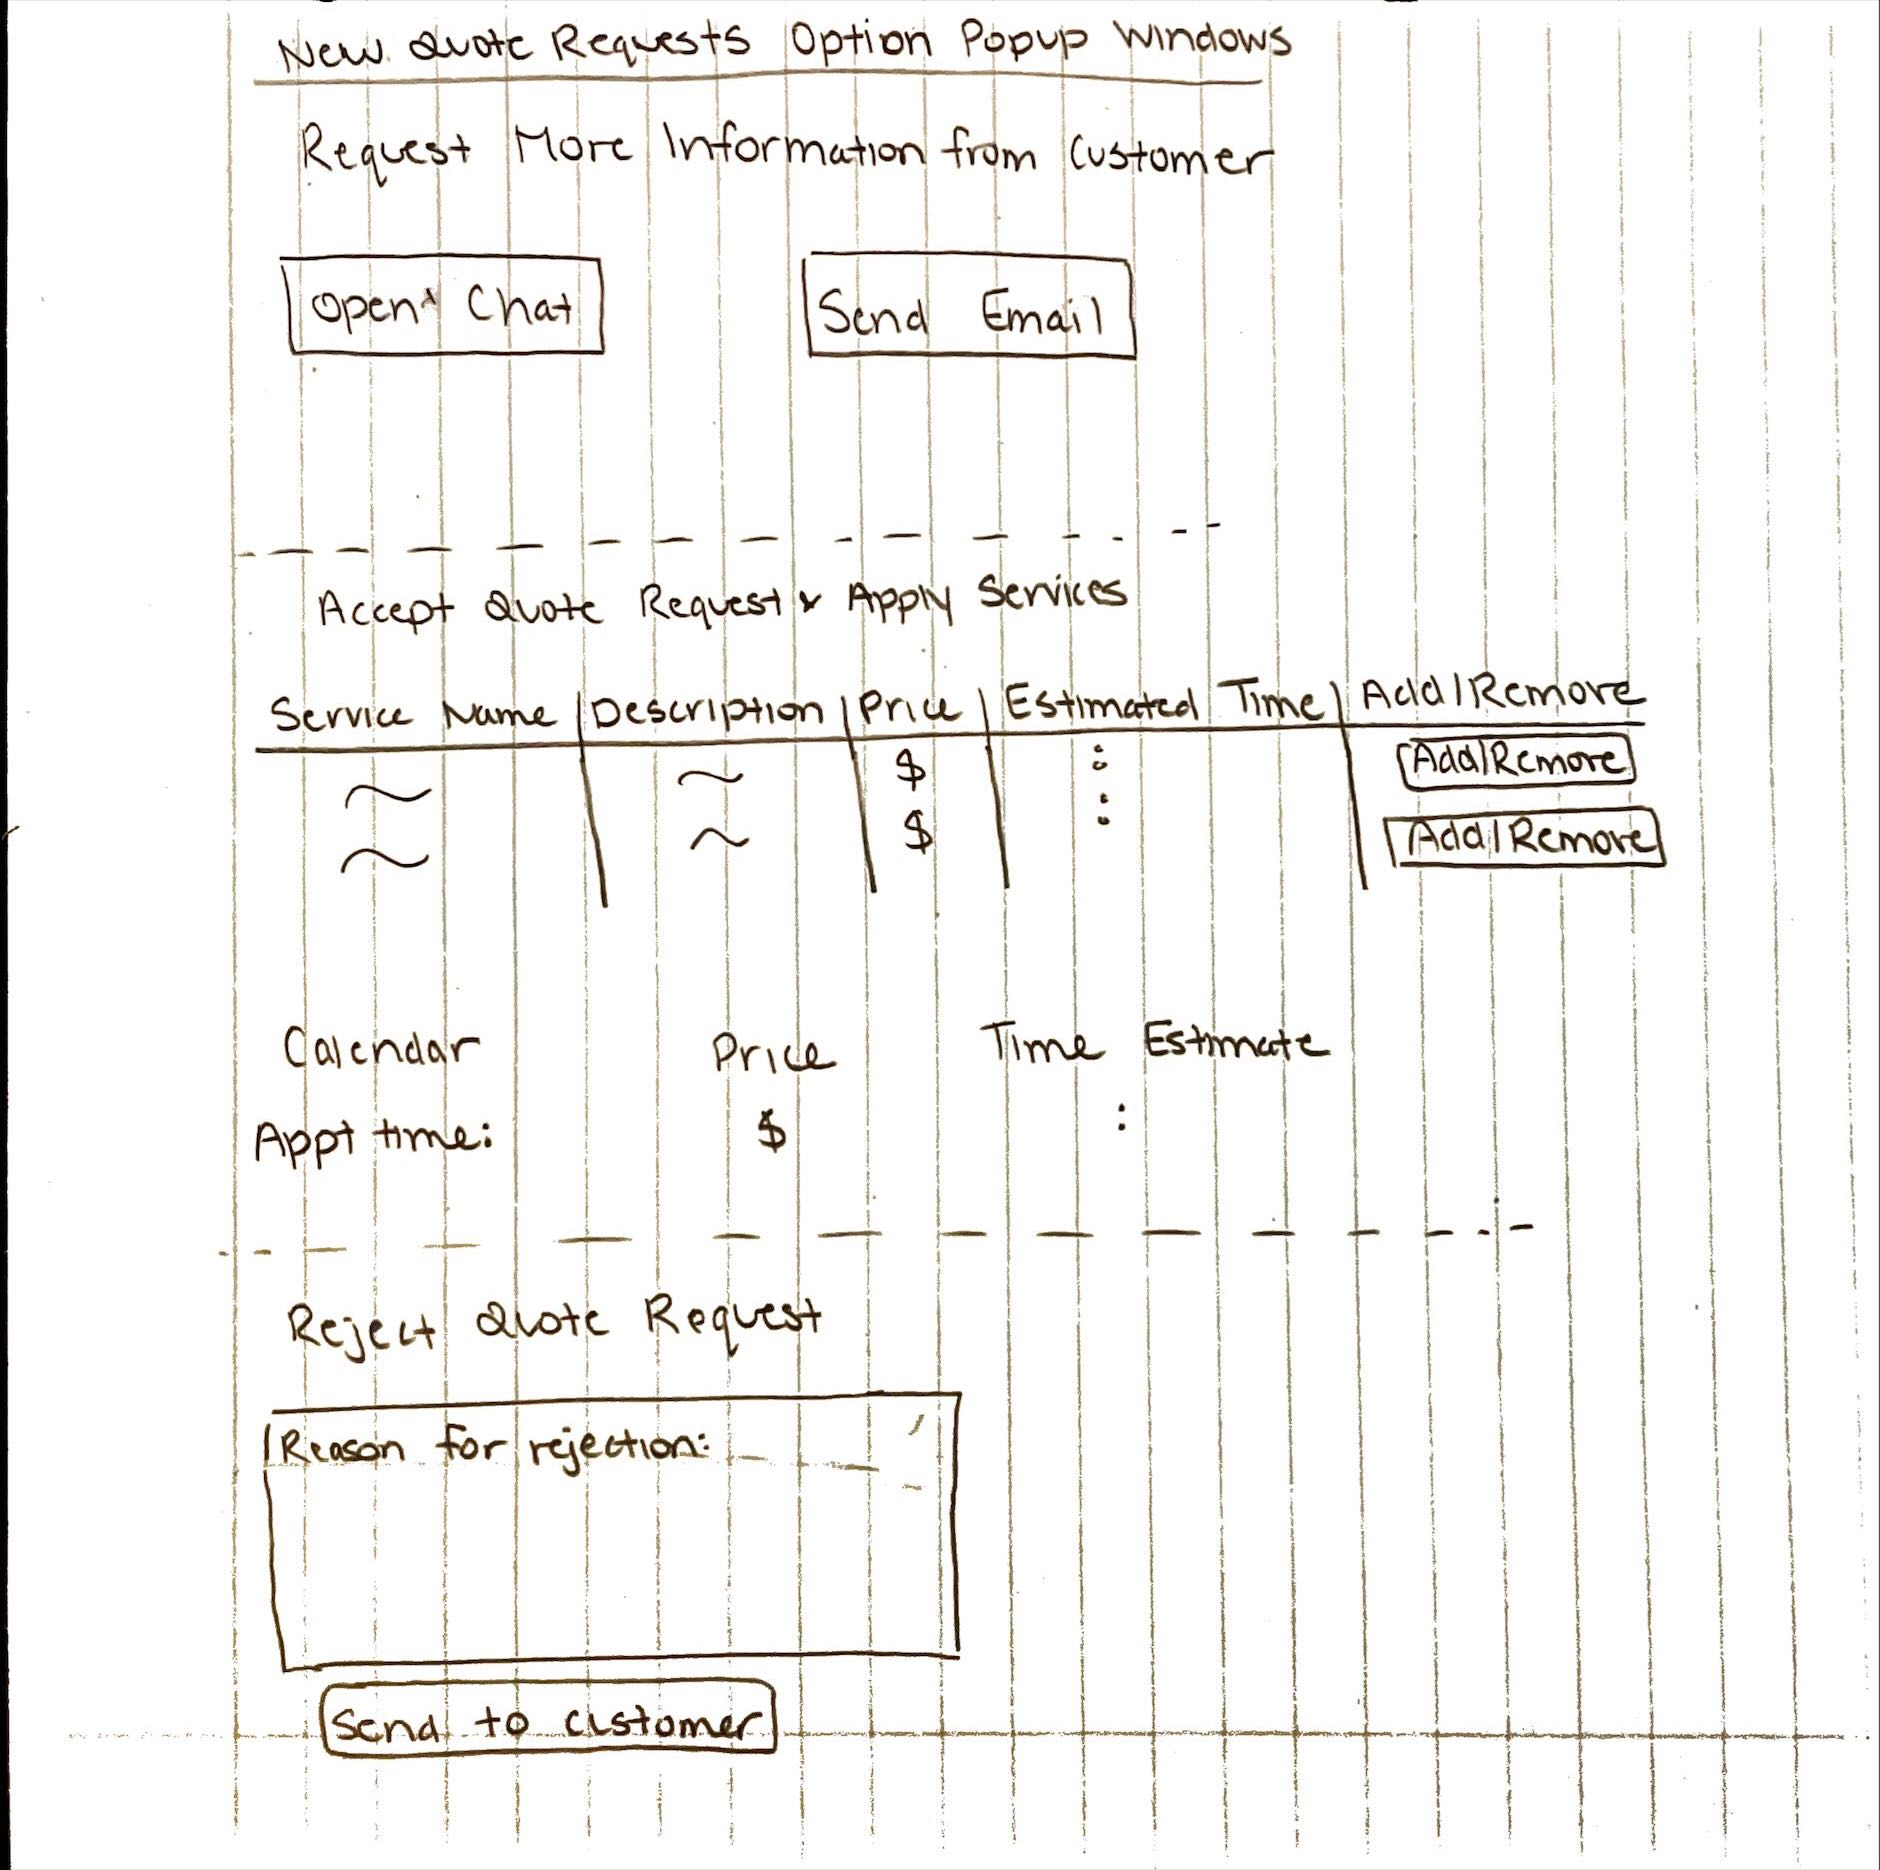
\includegraphics[width=\textwidth]{Design/SystDesign/Quotes/Quote3.png}
    \caption{Shop quote UI for each individual button pressed from \ref{quoteUI2}. Each menu is a separate popup that appears when the user clicks any one of the buttons.}
    \label{fig:quoteUI3}
\end{figure}

\begin{figure}[H]
    \centering
    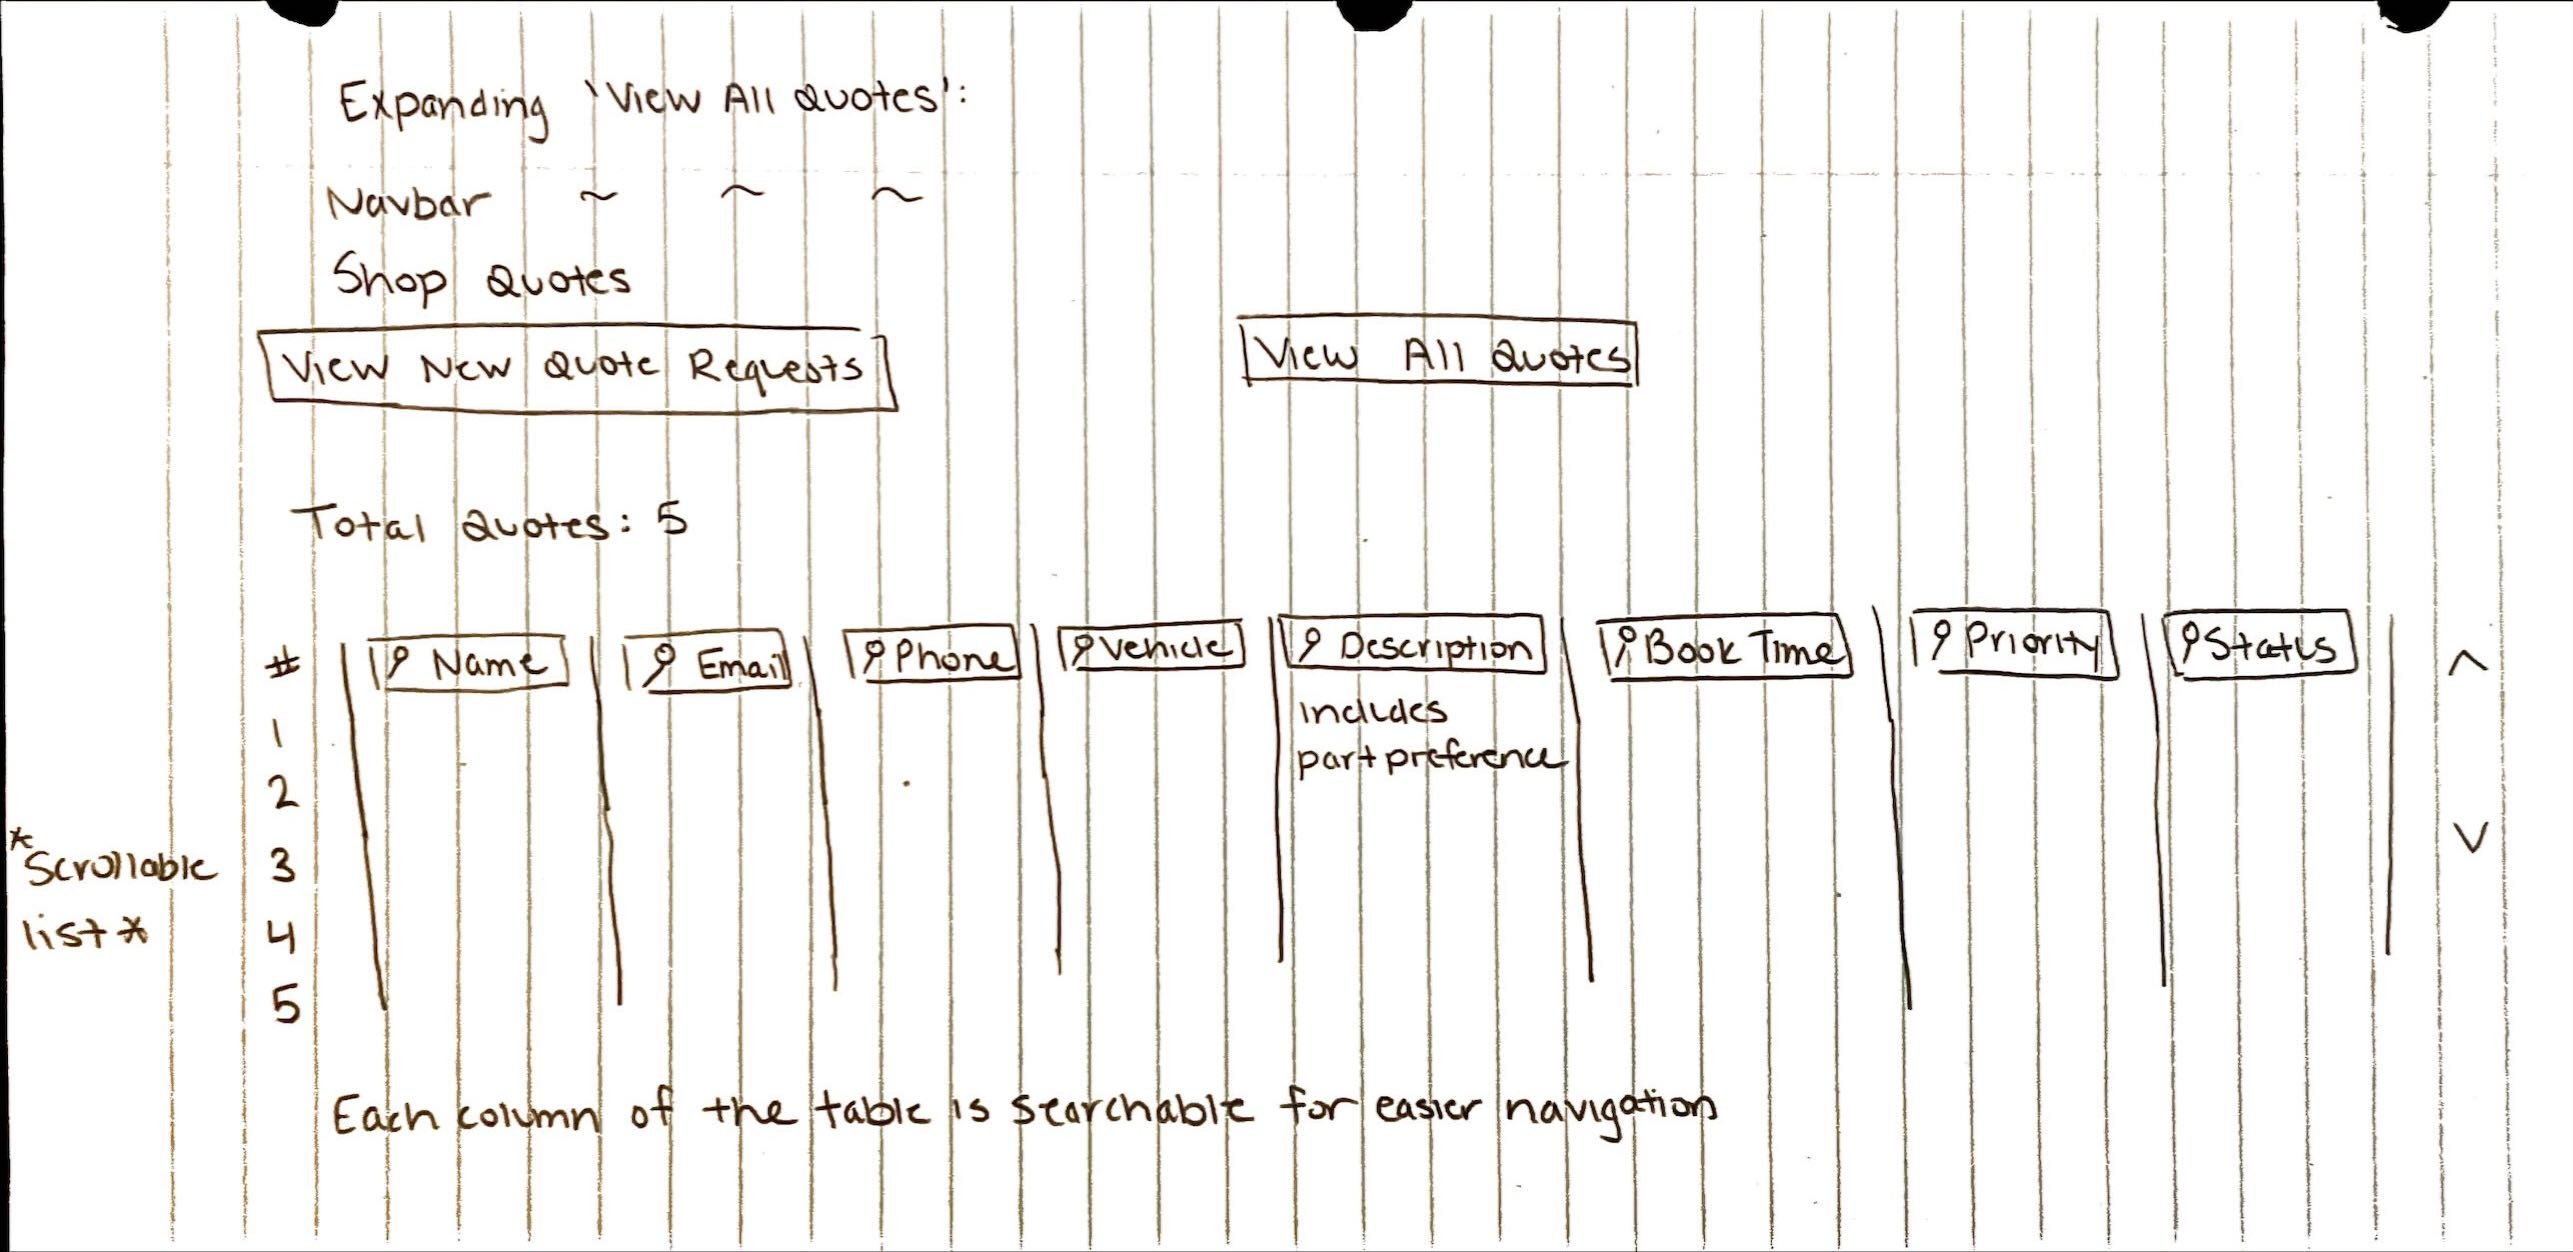
\includegraphics[width=\textwidth]{Design/SystDesign/Quotes/Quote4.png}
    \caption{Shop quote for UI when the user selects 'View All Quotes'. A searchable table by field appears for easier navigation.}
    \label{fig:quoteUI4}
\end{figure}

\subsection{ShopCreate UI}
\begin{figure}[H]
    \centering
    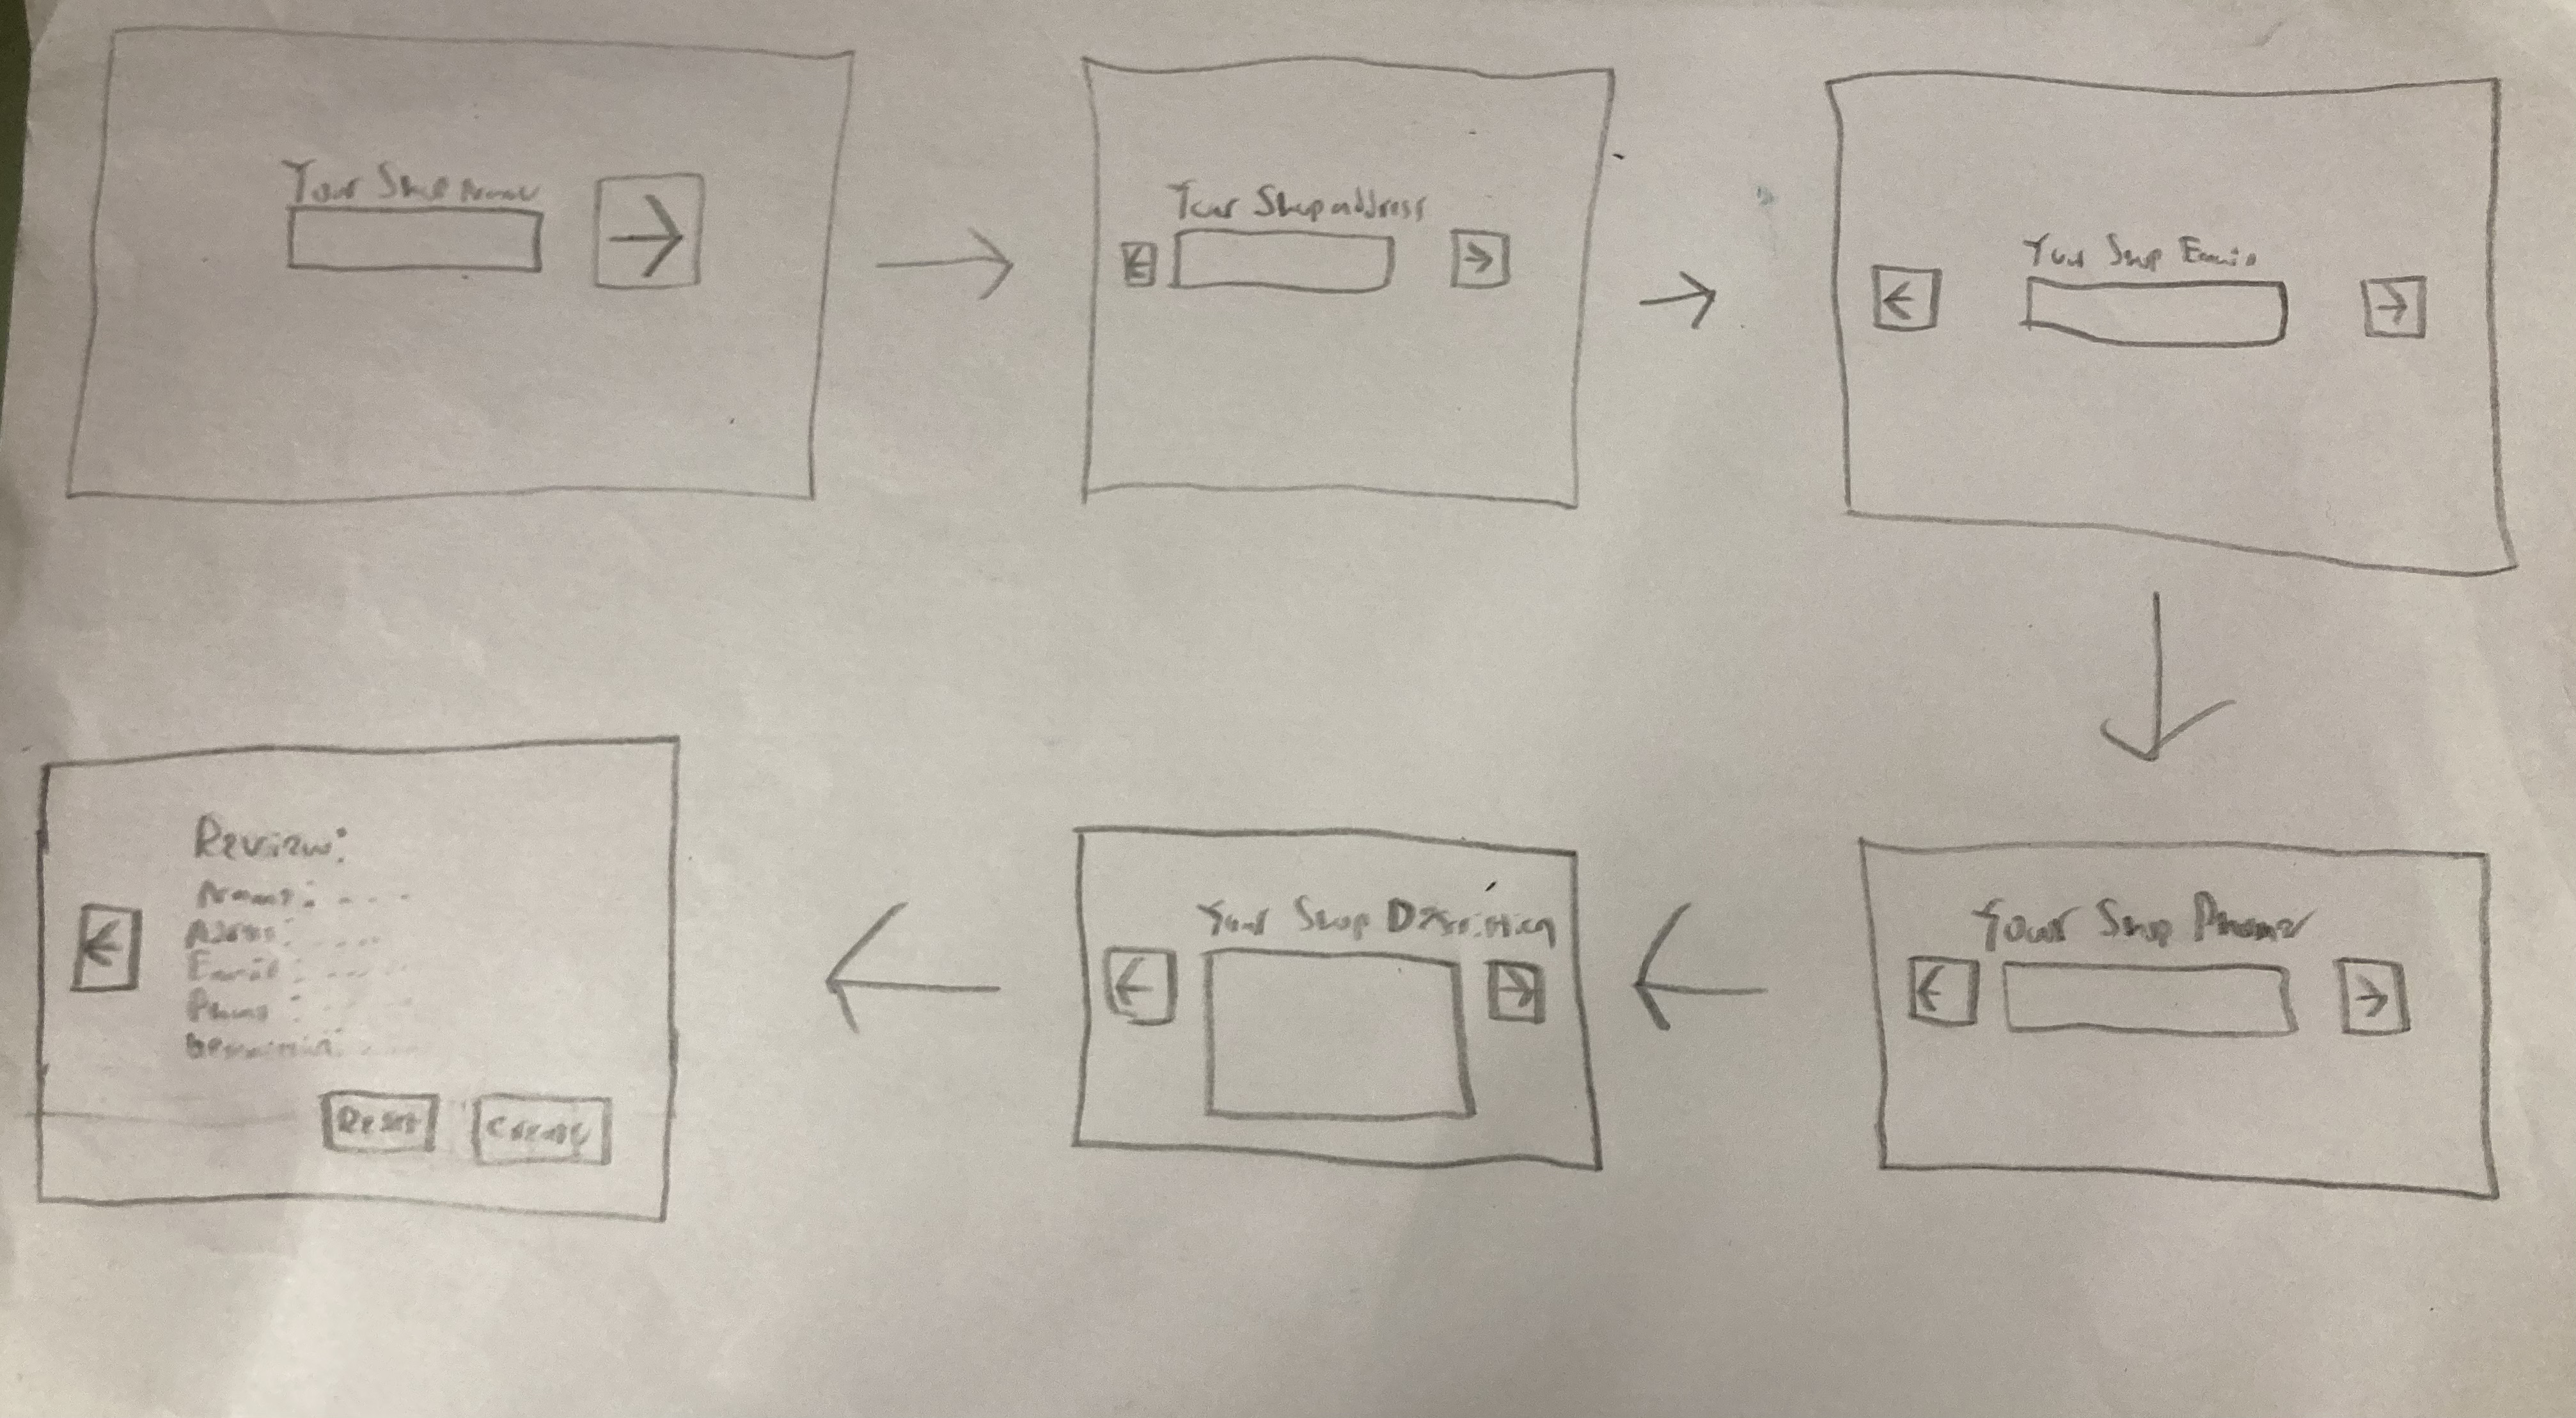
\includegraphics[width=\textwidth]{Design/SystDesign/ui_ShopCreate.jpeg}
    \caption{Displayed when a Shop Owner account first logs in, the UI features a single-page with sliding transitions per required field, allowing the user to create a shop in the backend}
    \label{fig:ShopCreateUI}
\end{figure}

\subsection{ShopLookup UI}
\begin{figure}[H]
    \centering
    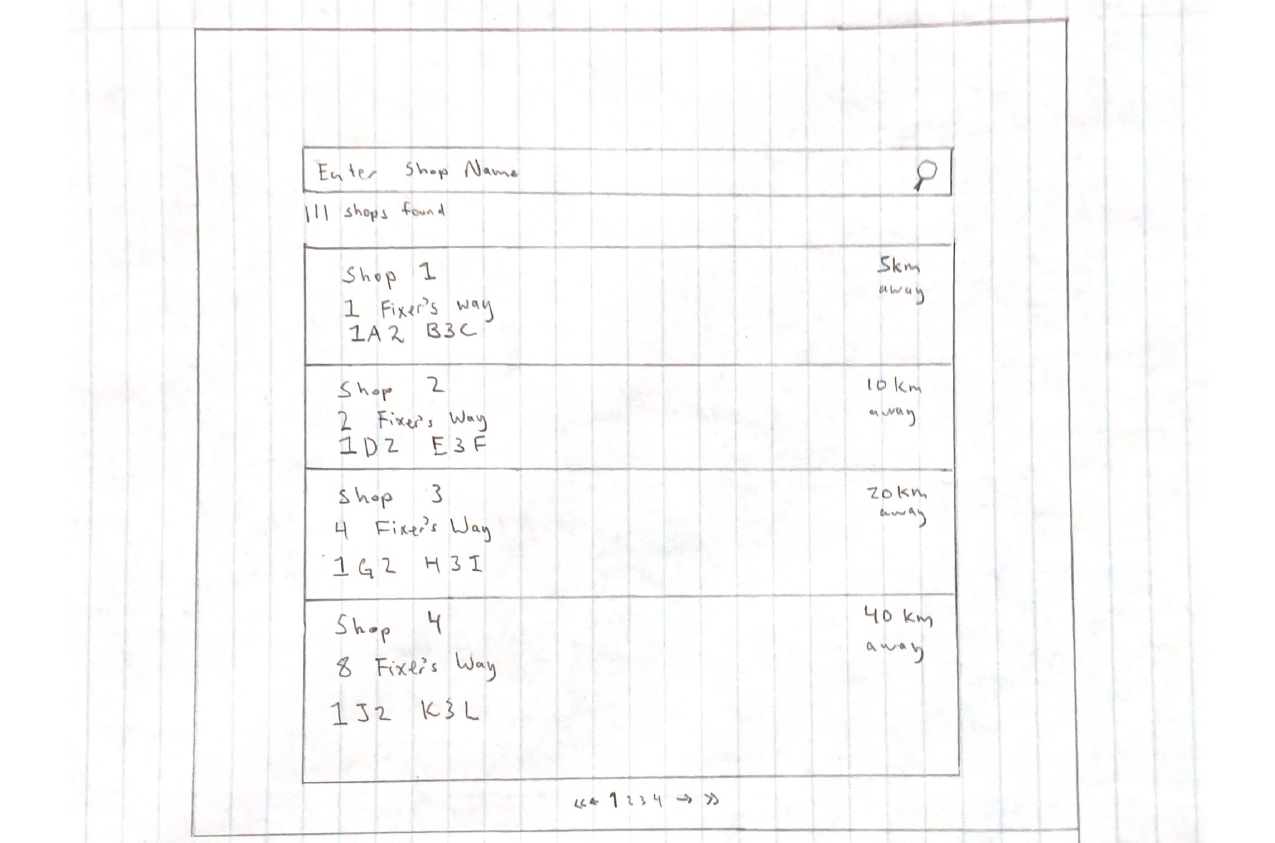
\includegraphics[width=\textwidth]{Design/SystDesign/ui_lookup.jpg}
    \caption{Displayed after clicking the navigation bar section labelled "Shop Lookup". Provides customers with all shop names in the database and allows them to filter by name, postal code, and distance by searching. Clicking a search result brings them to a page with more details of the shop, including shop services.}
    \label{fig:shopLookupUI}
\end{figure}

\subsection{Homepage UI}
\begin{figure}[H]
    \centering
    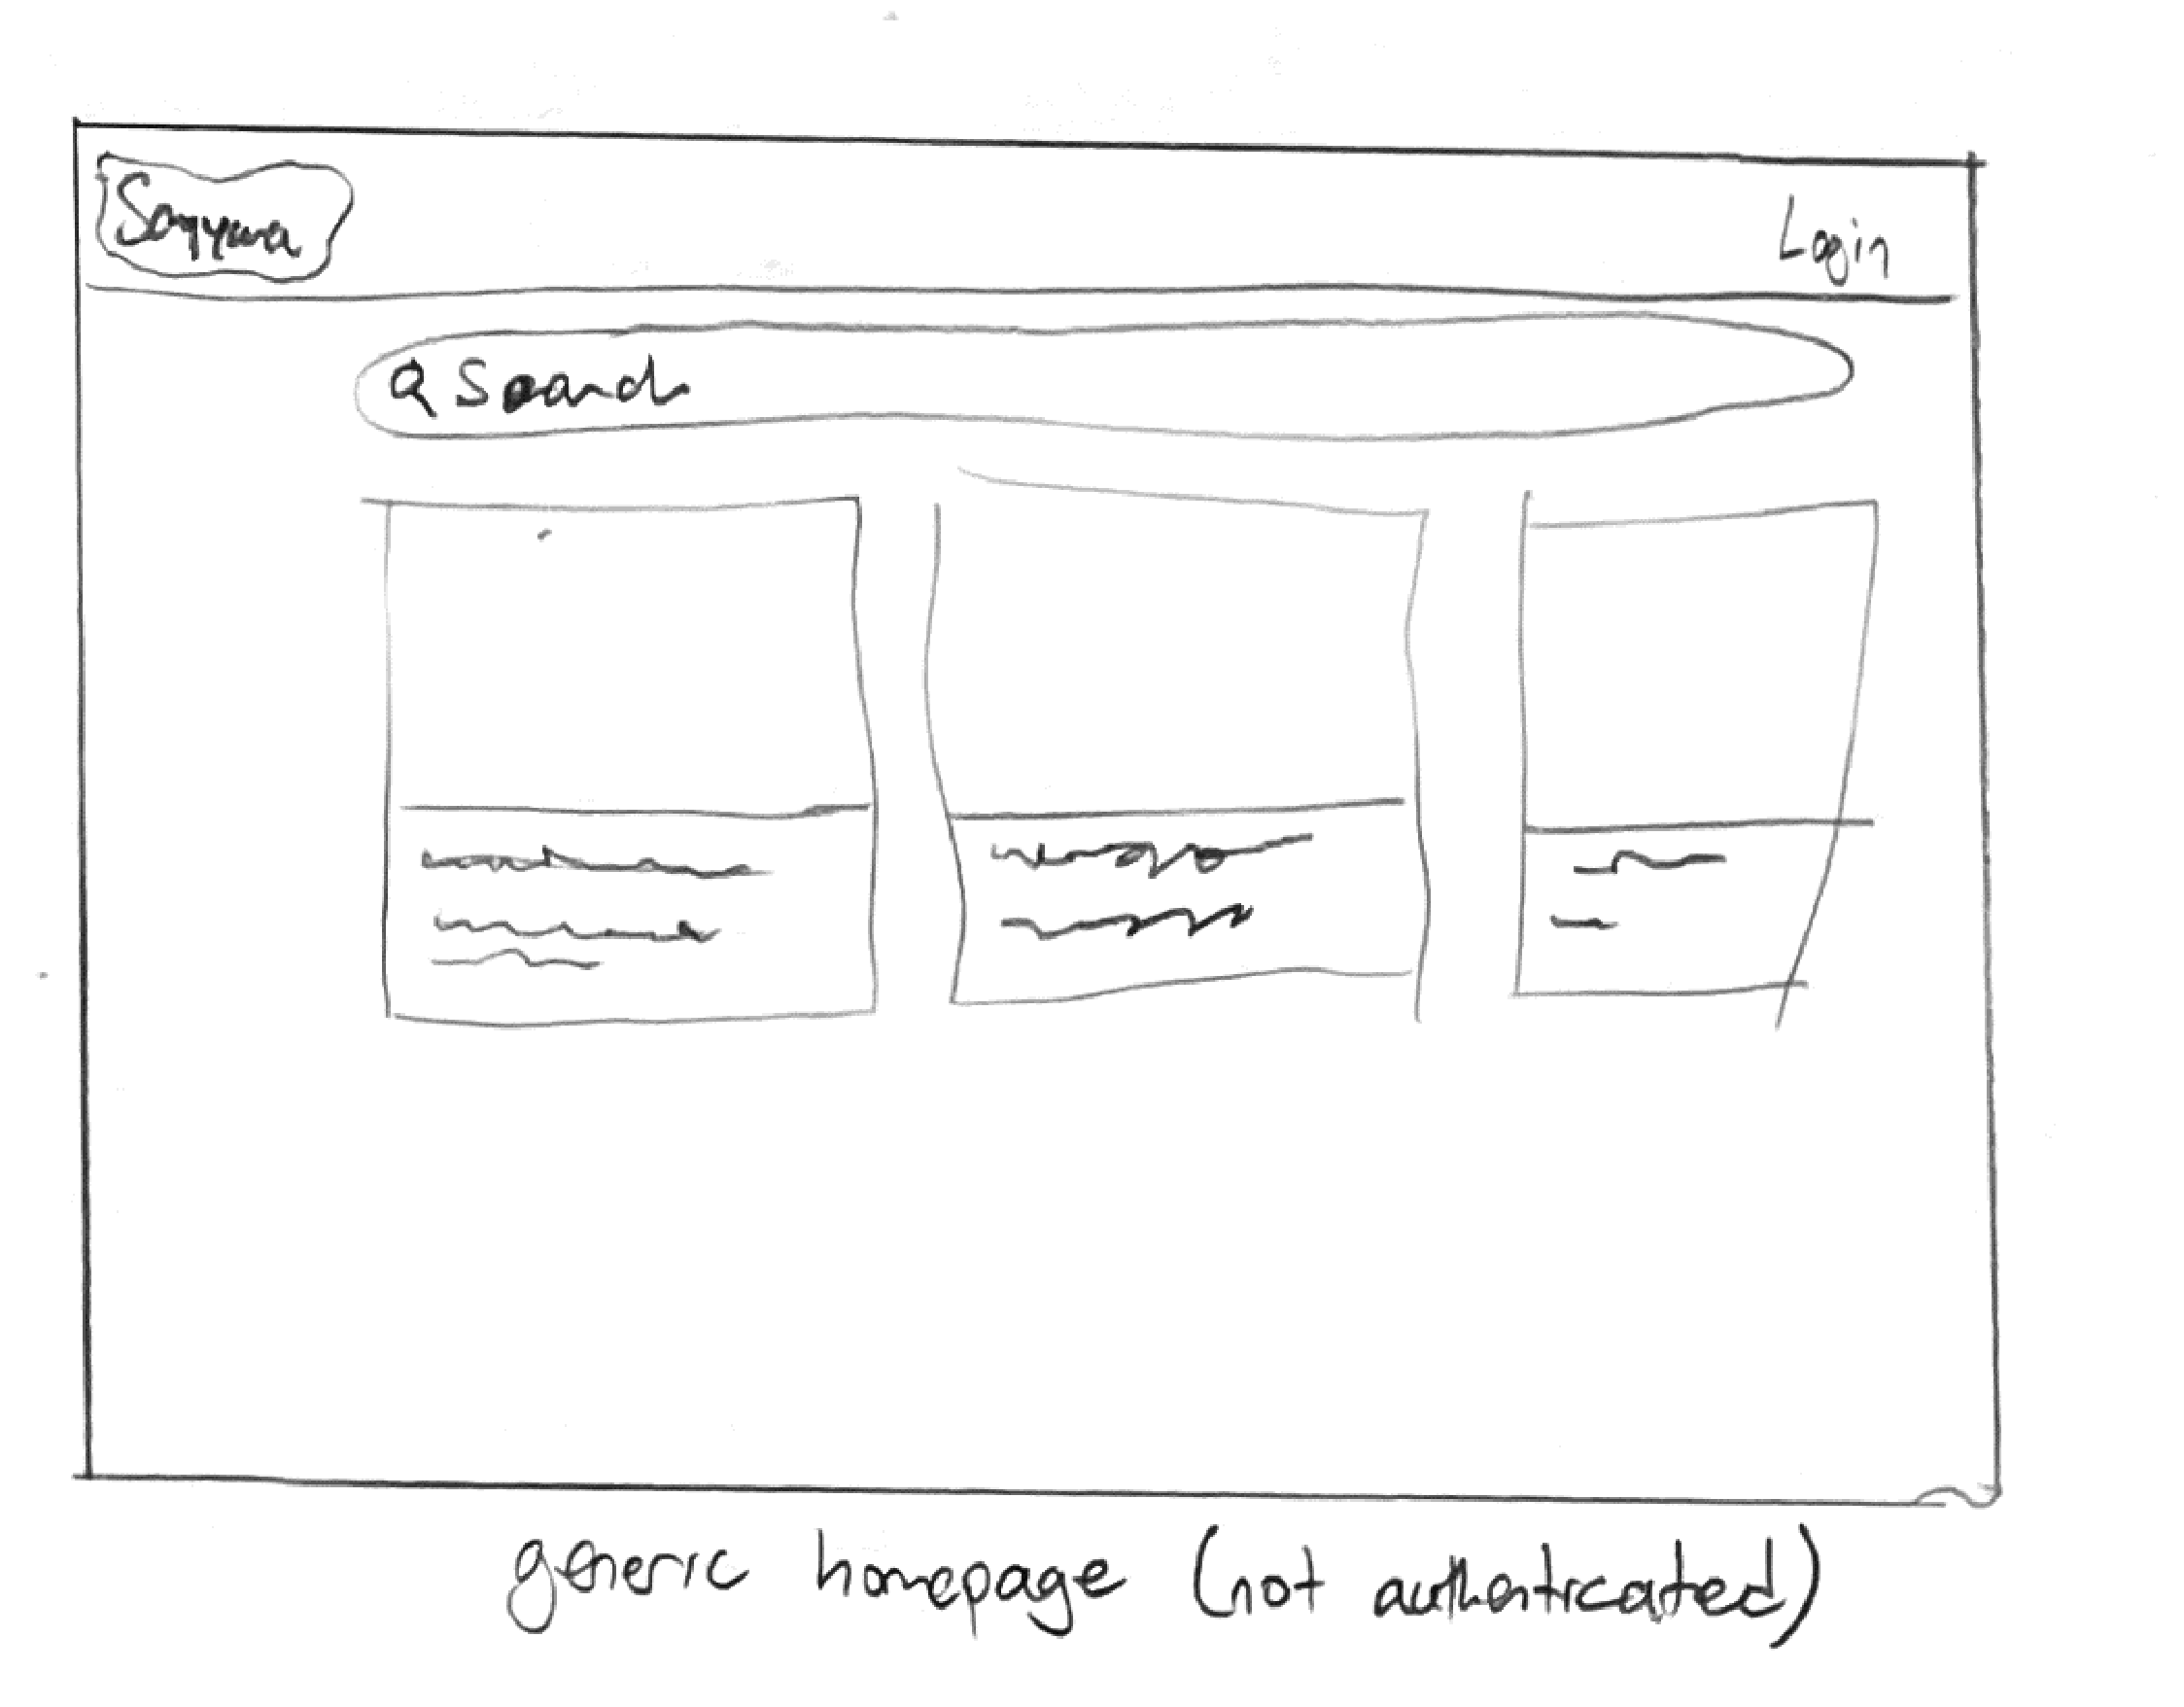
\includegraphics[width=0.5\textwidth]{Design/SystDesign/homepages/ui_genericHome.png}
    \caption{Generic Homepage for users who are not authenticated}
    \label{fig:genericHomepage}
\end{figure}

\begin{figure}[H]
    \centering
    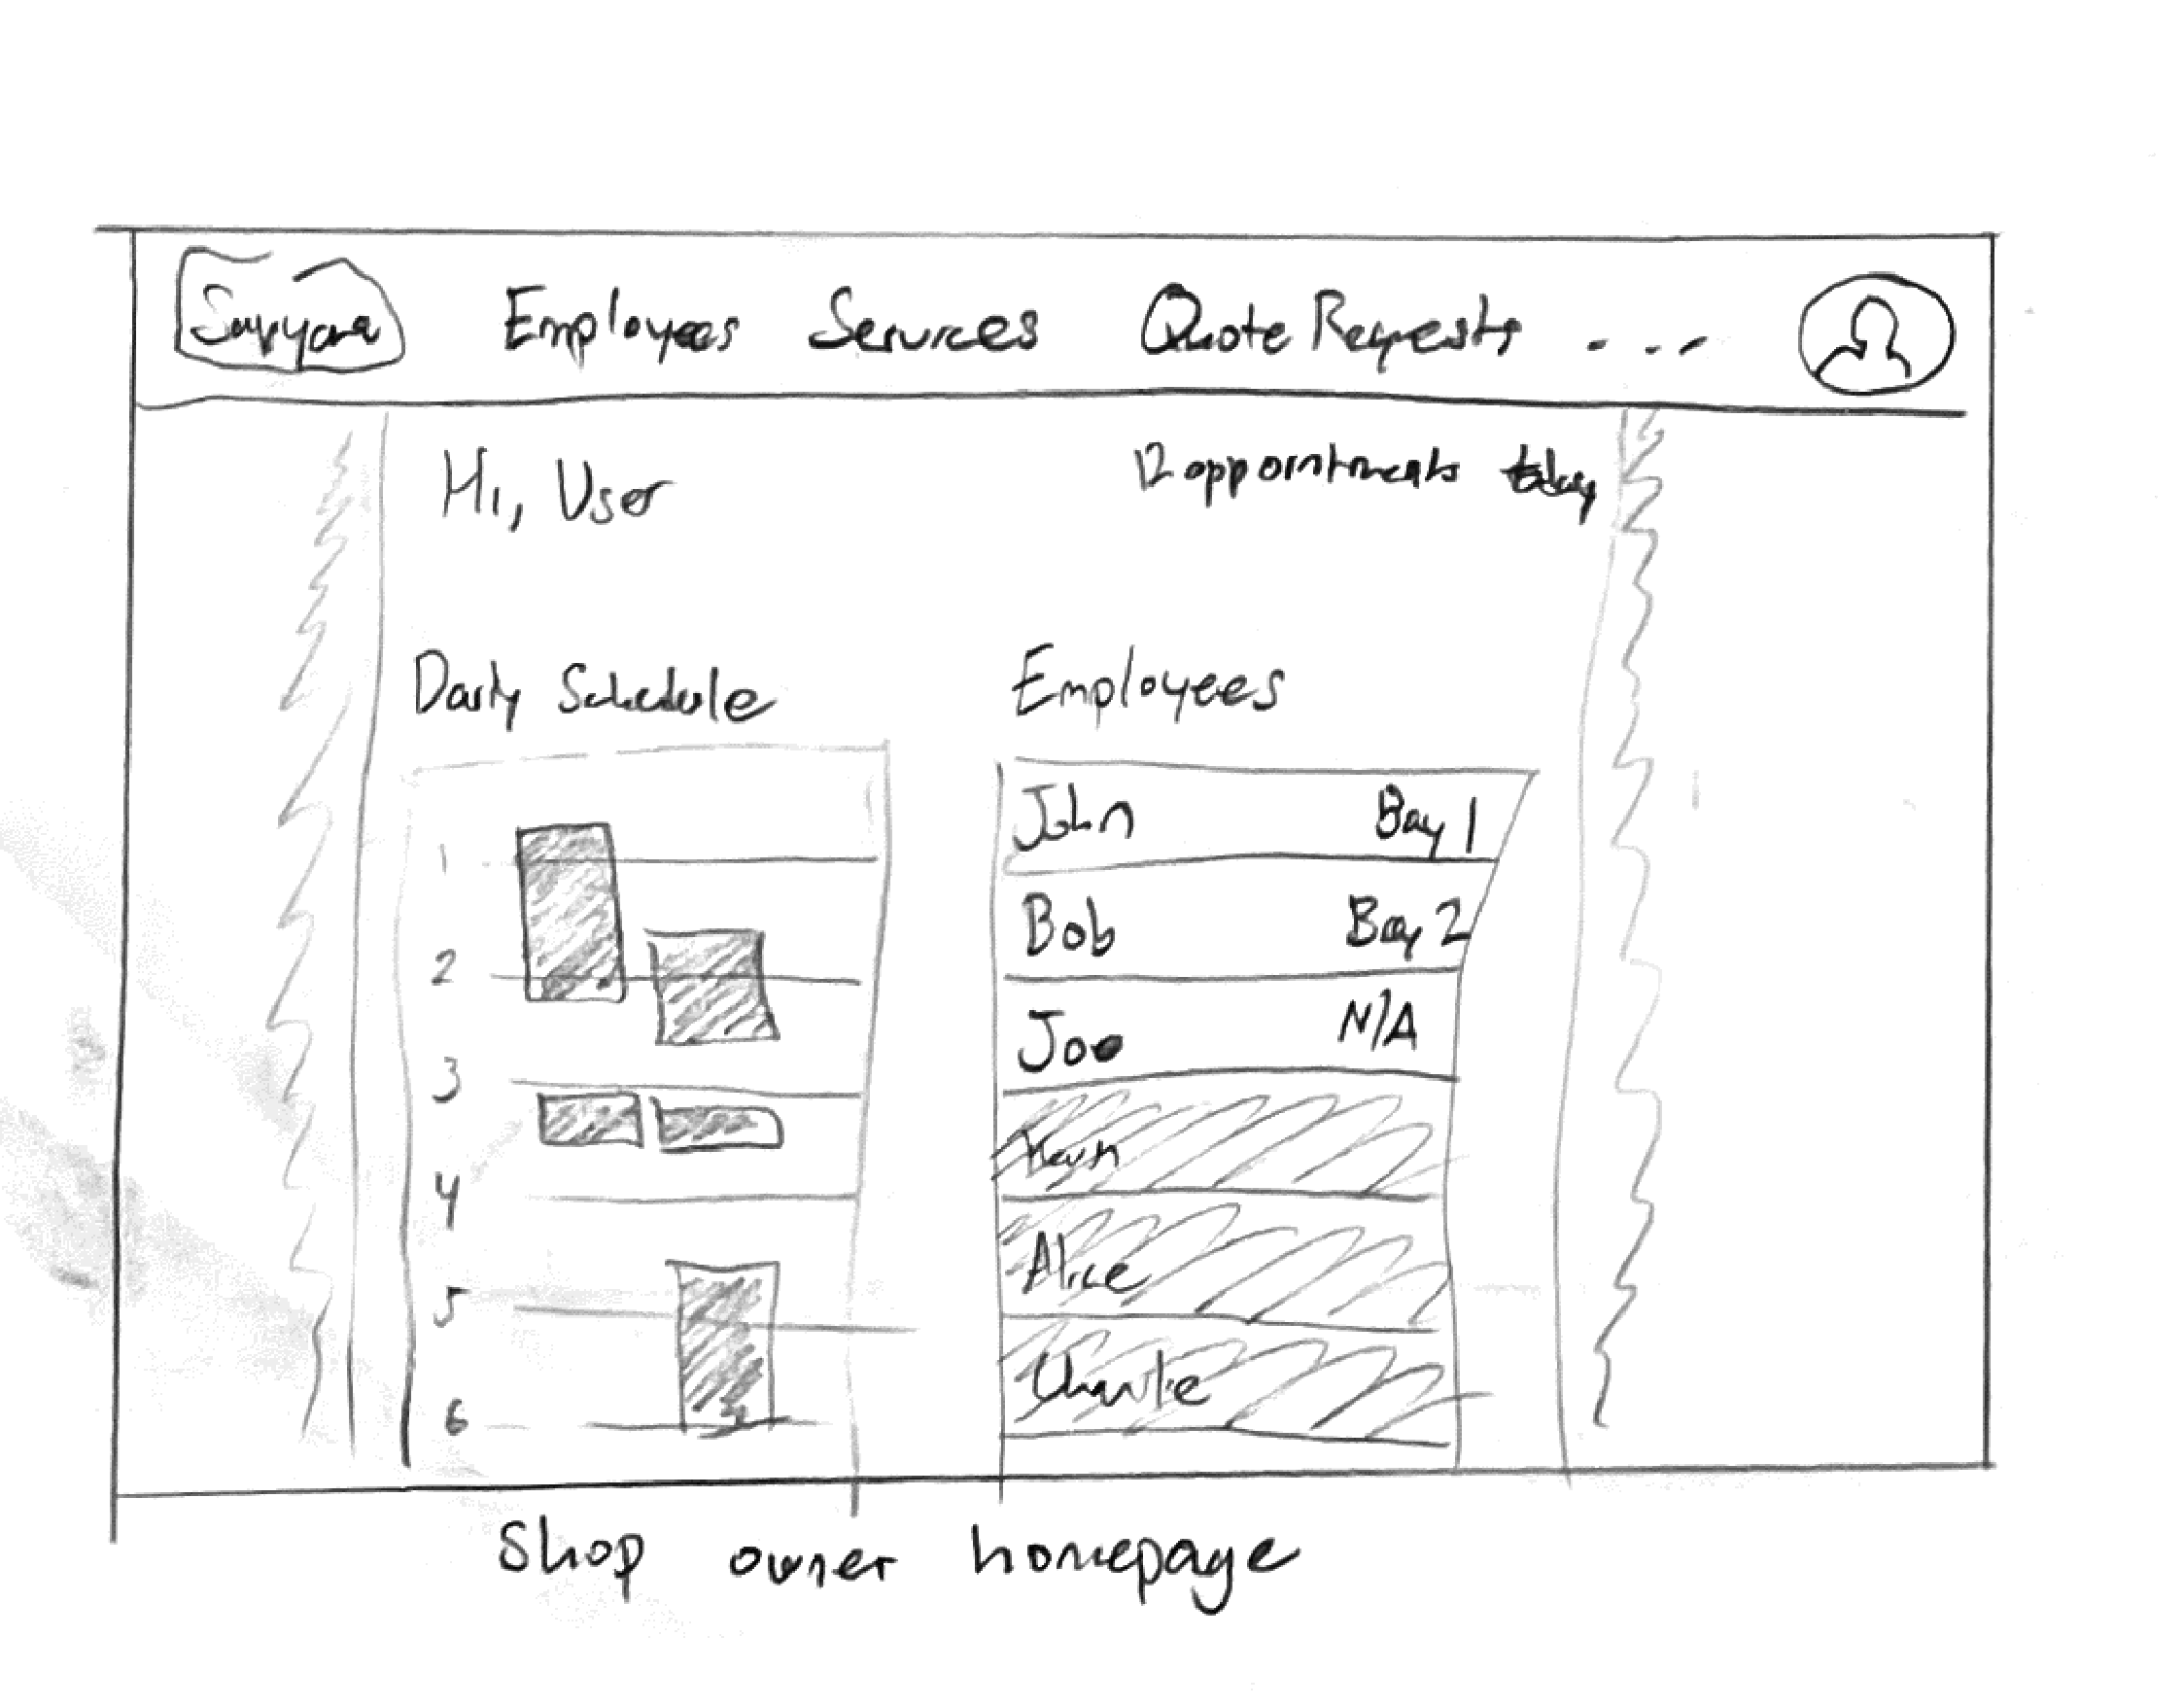
\includegraphics[width=0.5\textwidth]{Design/SystDesign/homepages/ui_ownerHome.png}
    \caption{Homepage with shop owner specific information included}
    \label{fig:ownerHomepage}
\end{figure}

\begin{figure}[H]
    \centering
    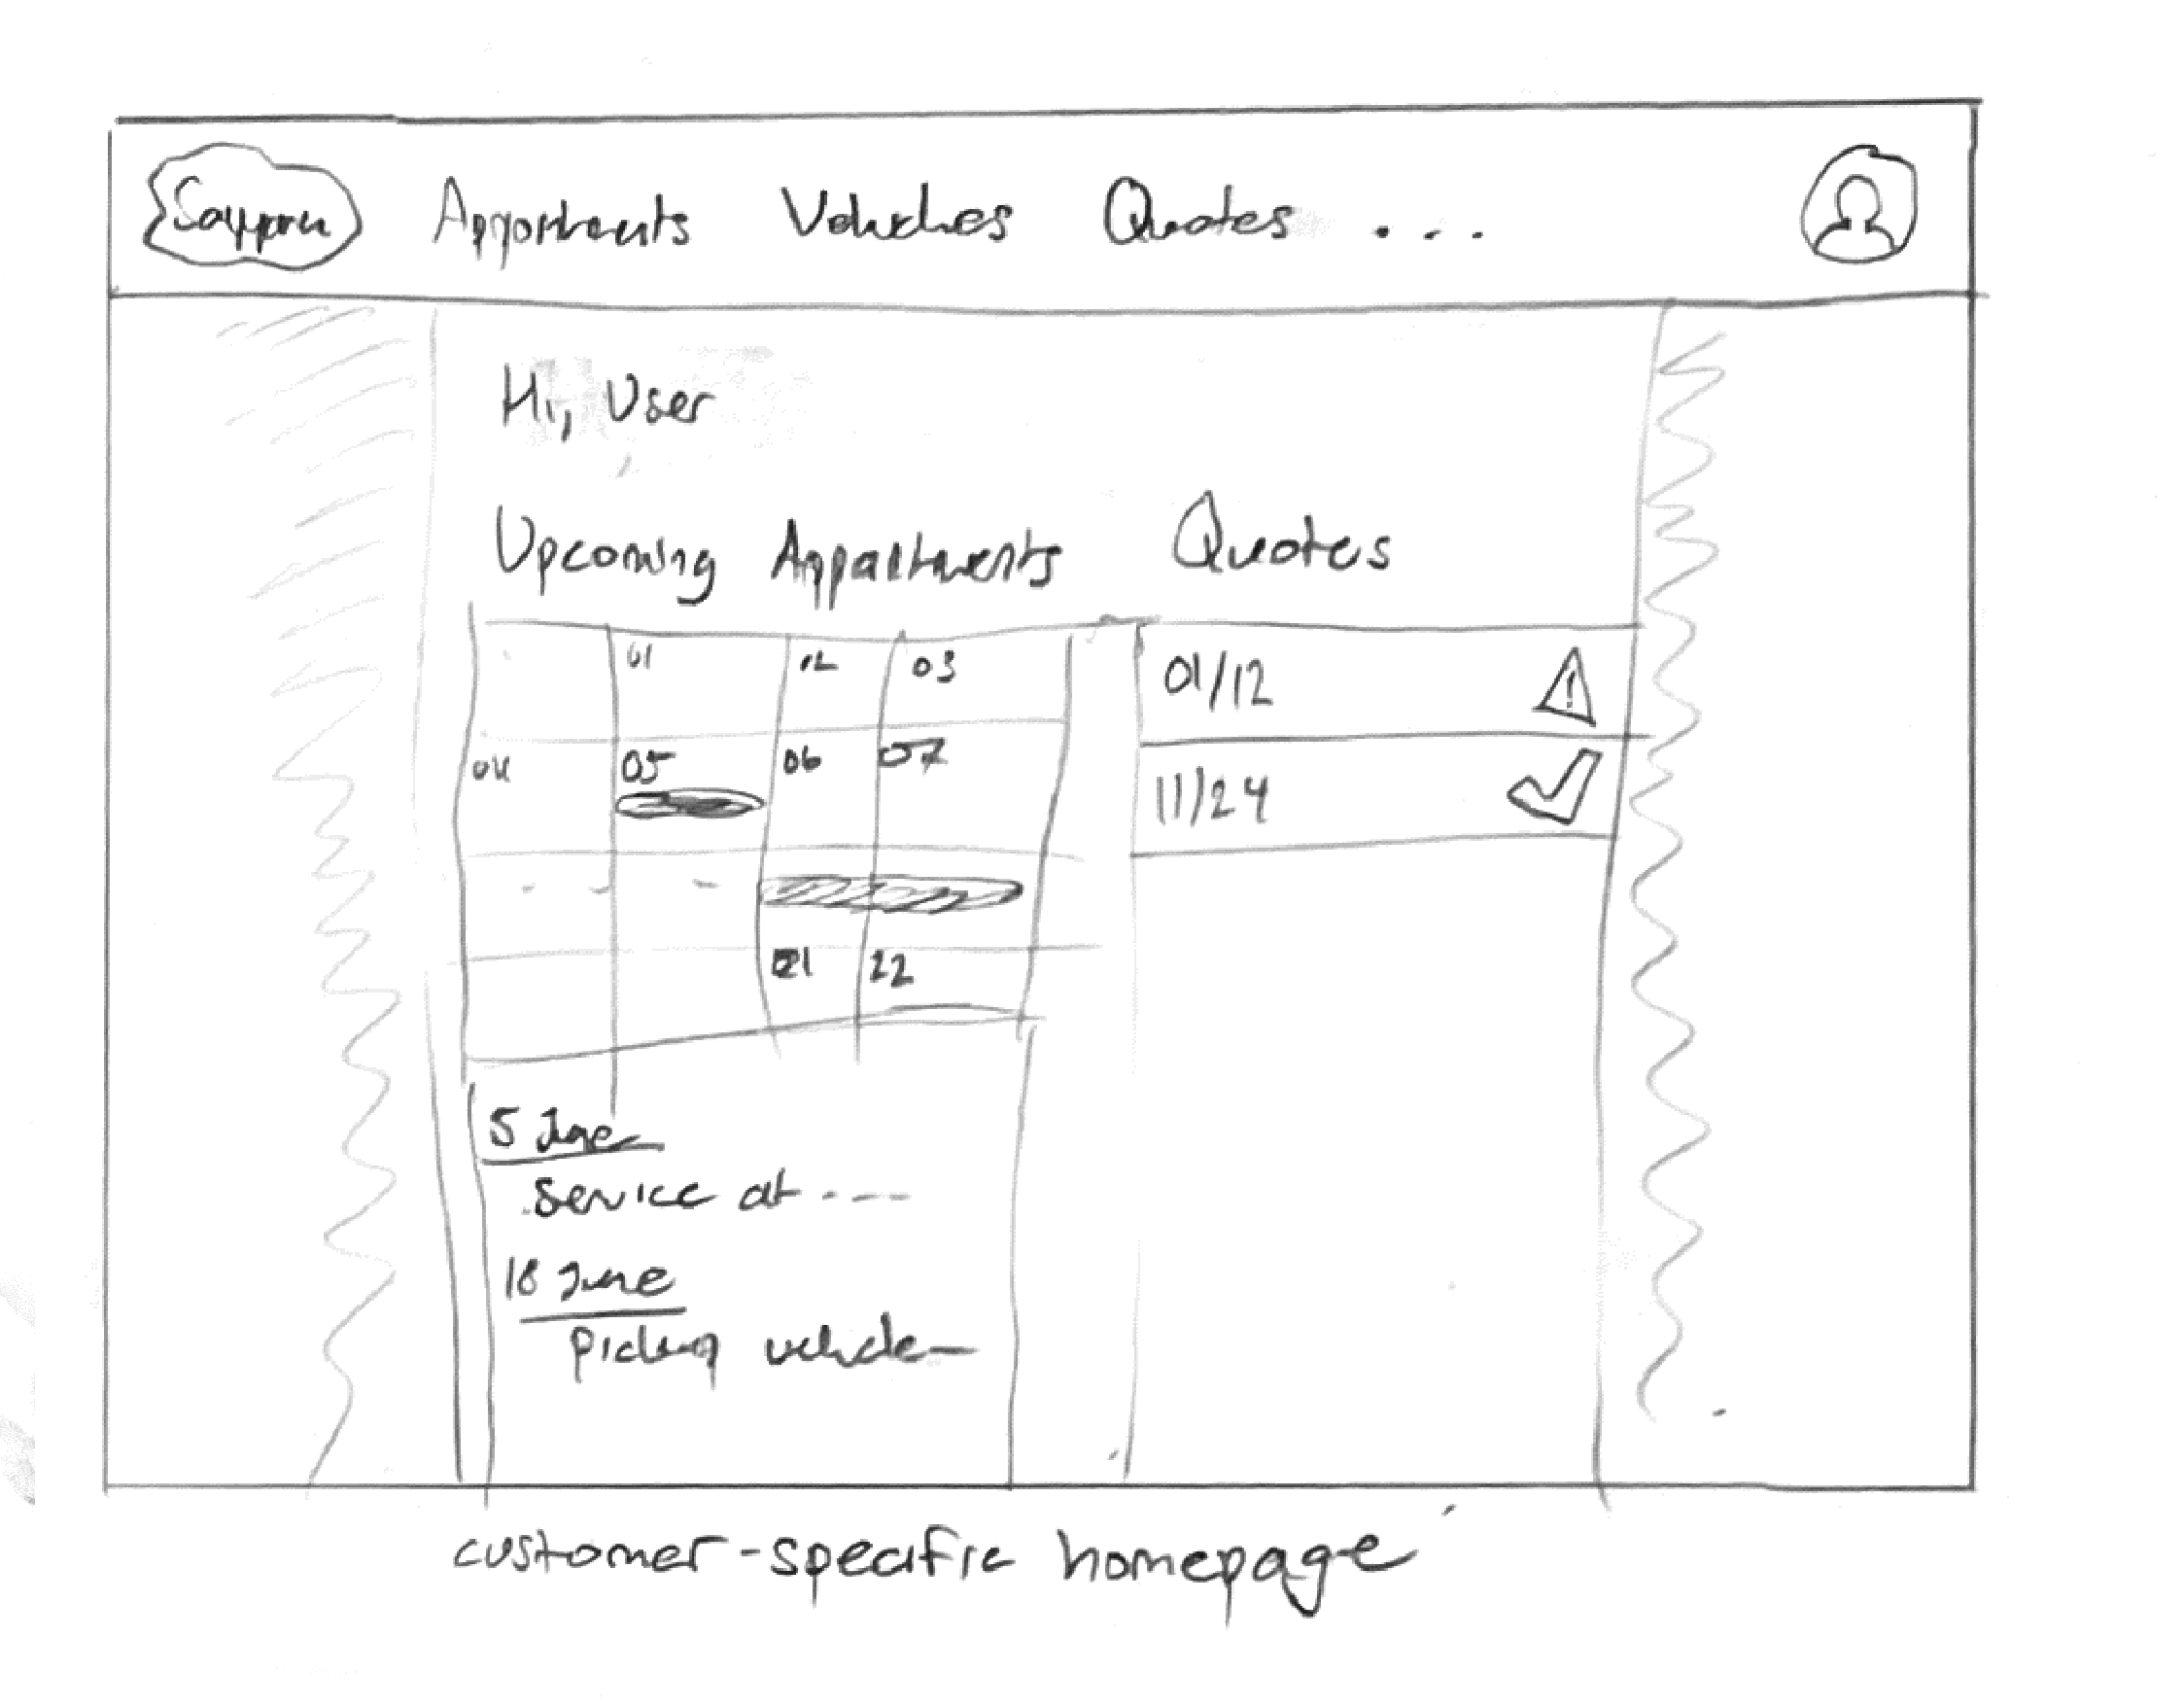
\includegraphics[width=0.5\textwidth]{Design/SystDesign/homepages/ui_custHome.png}
    \caption{Homepage with customer specific information included}
    \label{fig:custHomepage}
\end{figure}

\subsection{Profile UI}
\begin{figure}[H]
    \centering
    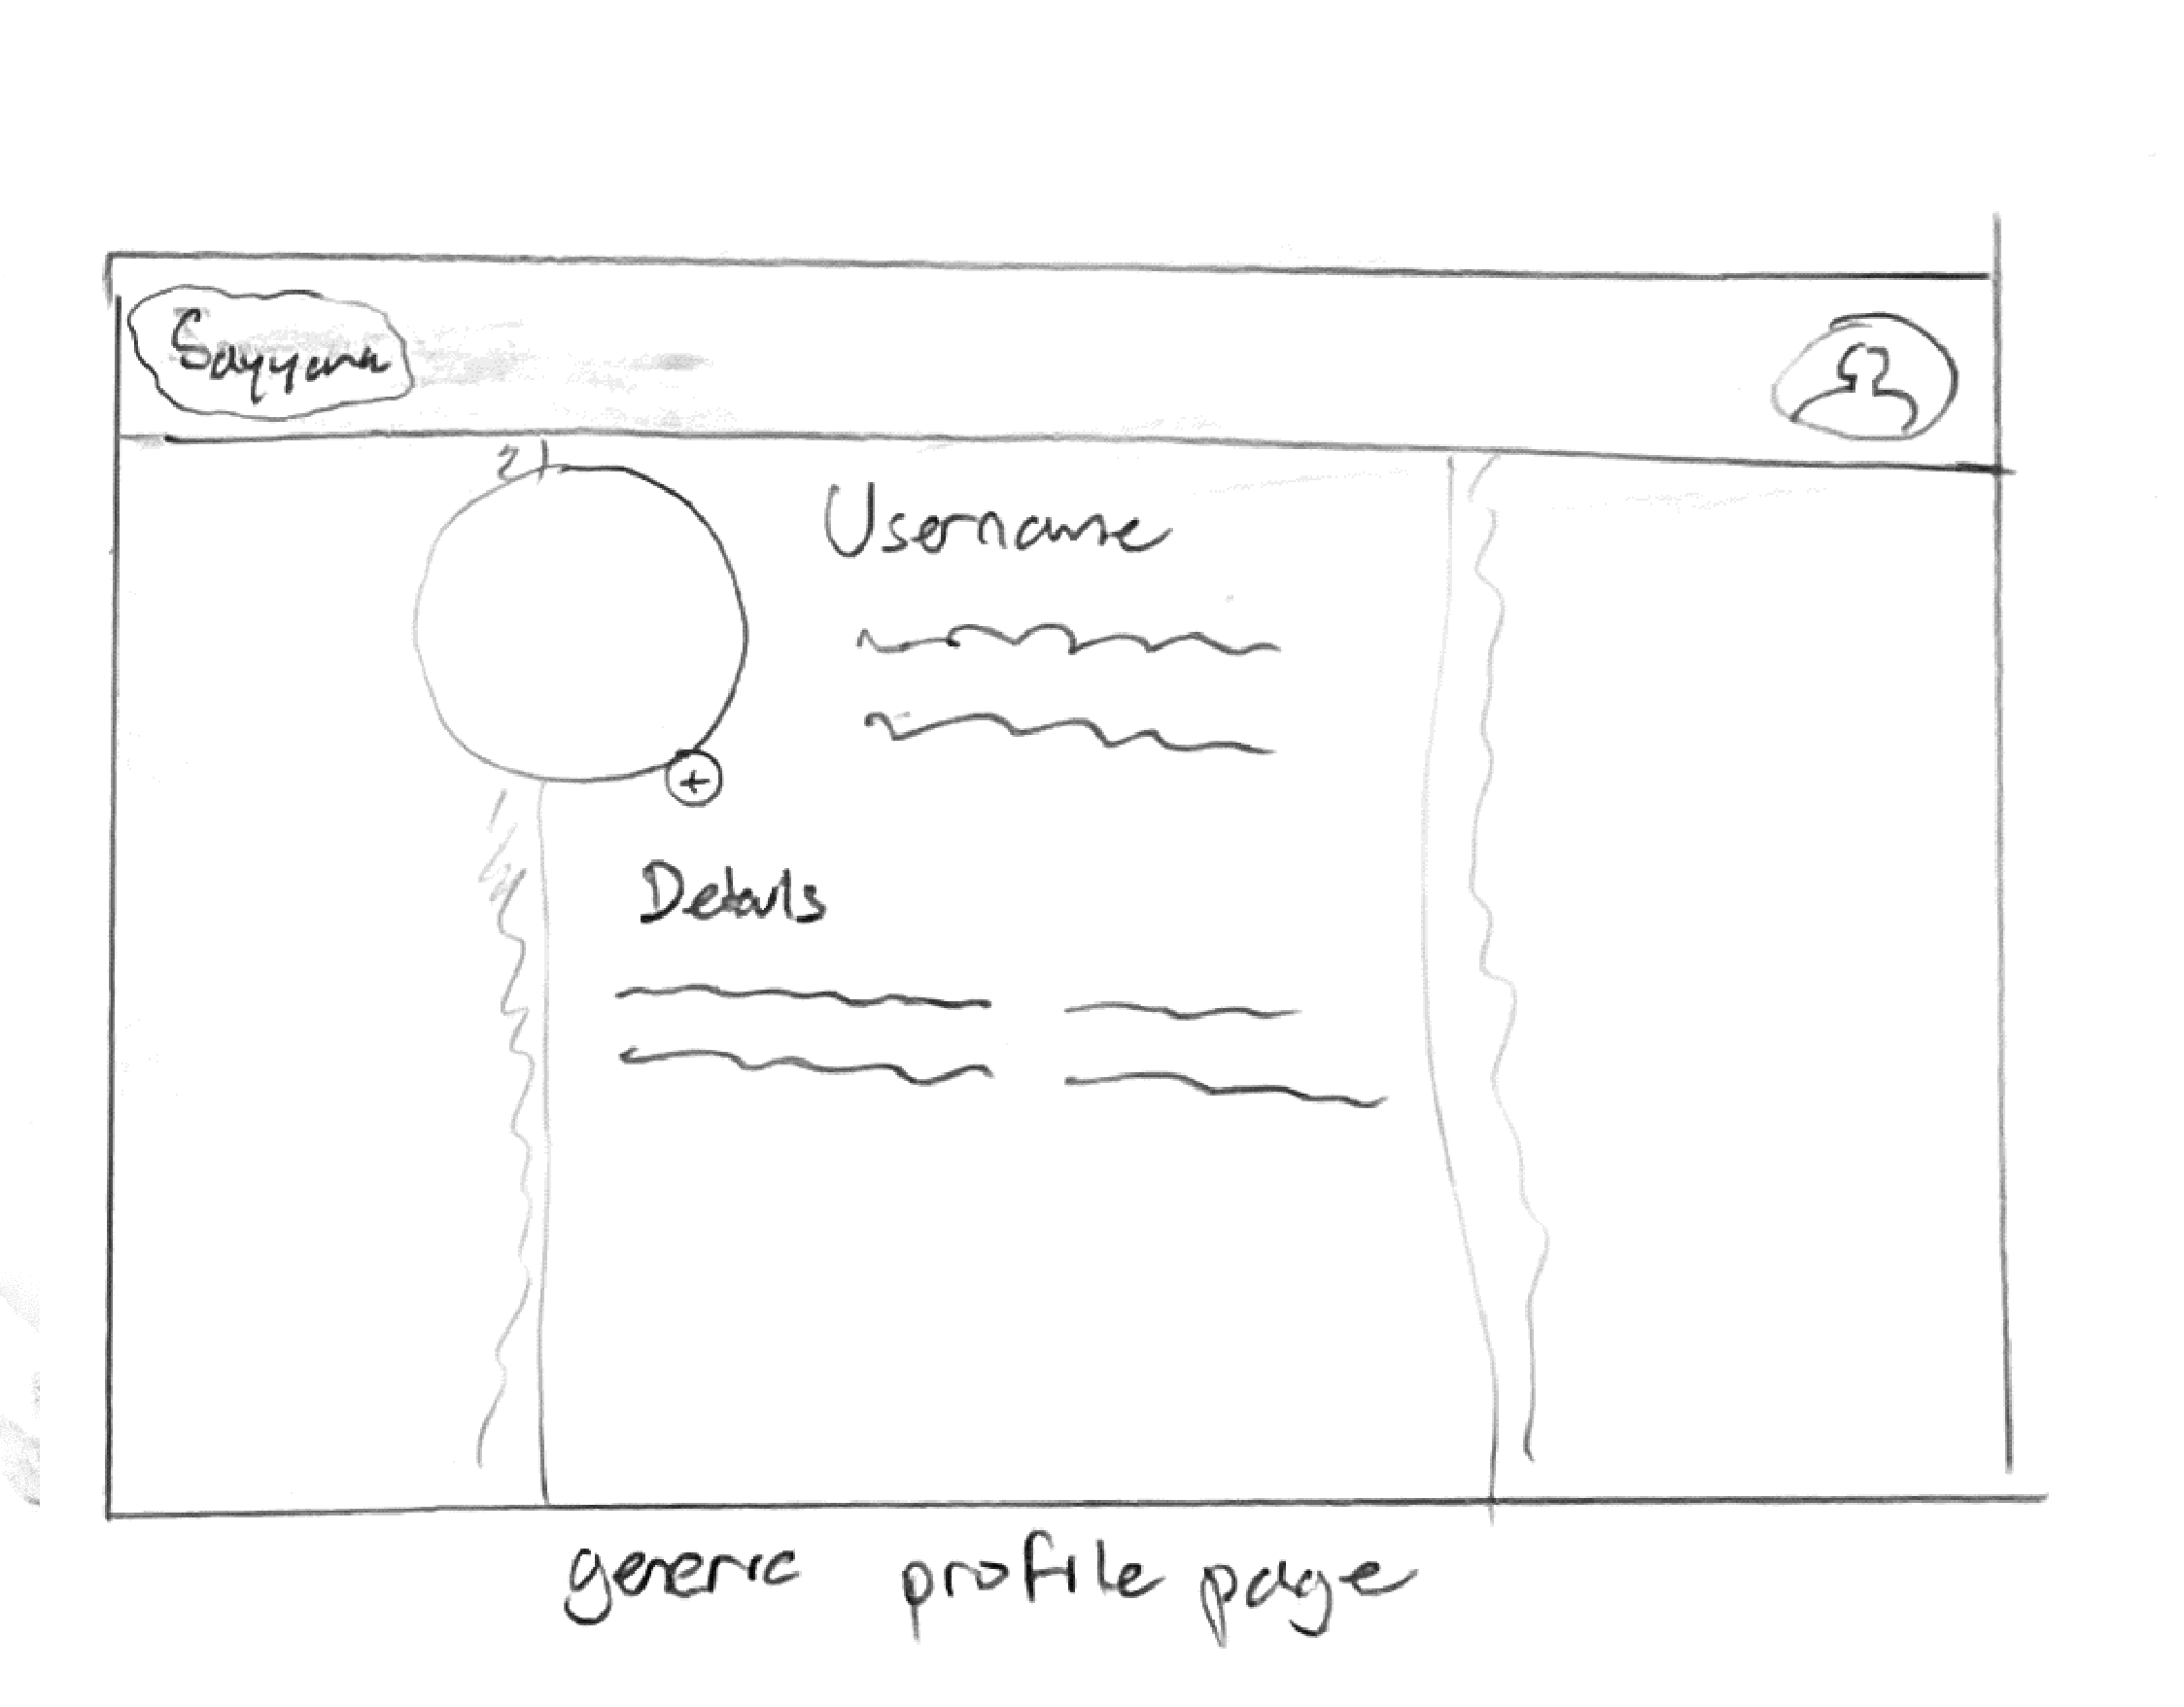
\includegraphics[width=0.5\textwidth]{Design/SystDesign/homepages/ui_genericPro.png}
    \caption{Generic profile page layout}
    \label{fig:gnericProfile}
\end{figure}

\section{Mechanical Hardware}

N/A

\section{Electrical Components}

N/A

\section{Communication Protocols}

\section{Reflection}

The information in this section will be used to evaluate the team members on the
graduate attribute of Problem Analysis and Design.  Please answer the following questions:

\begin{enumerate}
  \item What are the limitations of your solution?  Put another way, given
  unlimited resources, what could you do to make the project better? (LO\_ProbSolutions)
  \item Give a brief overview of other design solutions you considered.  What
  are the benefits and tradeoffs of those other designs compared with the chosen
  design?  From all the potential options, why did you select documented design?
  (LO\_Explores)
\end{enumerate}

Chris: \\
One limitation of the solution is that, as of the current plan, each Shop Owner can only create one shop. As listed out in the plan, the option for a Shop Owner to add an "Organization" consisting of many shops is a post-MVP feature, and there may not be sufficient time to add this feature; it would require much reworking on an already polished shop creation interface and backend. However, the design will be designed with maintainability in mind such that these features could reasonably be added afterwards. Another limitation is that fields like vehicle make, model, and year, as well as shop services, will be pre-defined dropdown selections from the backend. The reason this could be a limitation is because the User cannot enter a custom selection in the case that they feel none of the given selections accurately match what they are looking for. The team went for this design, however, because having pre-defined data types is easier to organize in the backend and display on the frontend, likewise making it easier for most users to fill in fields (pre-defined selections, if comprehensive, are often more straightforward).  \\

\noindent Another possible way the team could've designed the application is to merge Quotes, Work Orders, and Services, since they are all intertwined and essentially transform into one another. However, the team decided that it would be better to modularize these different components, especially because they may require more distinct information than anticipated, and it makes it easier to manage. Sometimes over-generalizing can have consequences of being difficult to use, and this likely would've been the case.

Alyssa: \\
One limitation, specifically for the Quote and QuoteRequest section of the application is the post-MVP idea to have a live chat service so that customers and shop employees and communicate in real time about any issues with quote requests or appointment scheduling. Due to time constraints and potential difficulty adding this feature, the team is planning on going with the solution of having a chat service, but not so much a real time service. If given unlimited resources such as time, this feature would be more fleshed out, but given it is post-MVP, a simpler implementation is planned. The solution we are considering, while simpler and potentially less effective at getting users to communicate with each other, still offers a way for users to communicate, but in a less timely manner than a complete live service. We believe this will be sufficient for the final revision.

Harsh:\\
One of the biggest limitations of the system is that there's no verification or validation in place to check if the data being sent by the frontend/backend is in the correct form with respect to the models. Moreover, given unlimited resources, it would be useful to make uses of TRPC or similar typed communication protocol to lock down the data structures that communicate between the backend and frontend.
Our current solution allows for the developers to setup a development environment locally which improves the overall commit cycle time. It also allows those who are interested in designing the frontend work independently of those working on the backend, which is scalable in-case this product were to go in production and be managed by multiple teams. One of the trade-offs with such a solution is the technical debt of running a Django + React stack, requires you to have developers who are experienced in at least one of these technologies. A monolith design on the other hand would be slightly less complex at the cost of higher commit cycle time because more people working and making changes to the same parts of the codebase requires more reviews, sometimes more technical debt depending on the teams' capabilities, and be tough to scale because of the tightly coupled components.
 
Kai:\\
The planned appointment scheduling system has a limited flexibility that does not accommodate certain scenarios. For example, scheduling availability is assigned in blocks of time, so if a shop has a one hour availability at the end of a workday, followed by an hour at the start of the next workday, the system would currently not allow the customer to book a two-hour appointment, despite it being a potentially desirable feature. Similarly, an intelligent scheduling system that books appointment into time slots that minimizes small blocks of unusable availability would be a very useful feature given more development time and resources.

Potential solutions to improve the flexibility and effectiveness of the scheduling include considering consecutive but disjointed (as described in the previous scenario) time as a single block of availability. This is, however, further complicated by the requirement that availability is dependent on shop hours, employee availability, and service bay availability. Another option to improve efficiency of scheduling is to treat it as a knapsack problem and use an optimization algorithm to suggest best booking times based on current availability and the number of hours the projected service would cost. Implementing the suggestion system may take time beyond the scope of the MVP, and ultimately may have questionable value in practice since customer preference likely overrides suggested booking time. As a compromise which combines usability with an achievable implementation timeline, we choose to define appointment availability as the intersection between store hours, employee schedule, and bay availability. Customers are able to request booking during an available time. The shop and the customer can further communicate in the booking system to adjust or finalize an ideal booking time for both parties.

Collin:\\
One limitation of our solution is the fact that is a progressive web app (PWA). Given an unlimited budget, I believe that creating a dedicated native app for our solution will improve the project in the long run. This is because while a PWA has many benefits over a native (mainly cost and development time), it does fall short in some key areas. One big one is push notifications. Push notifications are proven to be more engaging than other types of communications (e.g. email). Emails can sometimes be easily overlooked or missed. PWAs do support a form of push notifications however they are done through browsers and are not supported on iOS (nearly 50\% of all phone users). This means that access to push notifications for our system can improve the user experience. There are many modules in our system that require some communication to the user, including quotes, live chat, and appointment reminders. For quotes, shops can be instantly notified when a customer requested a quote, and customers can be instantly notified when a quote has been given. Limitations with the live chat feature (e.g. development time, employee availability to respond) can also be hugely mitigated, as both communicating parties can be notified when the other has responded and will not need to wait and stare at the screen for a response. Another benefit to using a native app would be access to native hardware. This means that the app can fully utilize better hardware and optimize performance for a smoother navigation experience for all users (faster page loading time, or calculations), however they are still limited by the backend API requests required to load real time data and their own latency.

The documented design was chosen because a PWA is many times more convenient than building a dedicated native app. PWA only requires on change to the website code base in order for users to be able to see those changes (as opposed to manually updating the native app). You also don't need to create an app that can support both platforms (Android and iOS), as well as avoiding the need to register the apps on their respective app stores. Our chosen solution allows all the development to happen on one environment and doesn't require the knowledge of developing on any specific platform as all modern devices support a web browser. This also means that the desktop version of the website does not need to be separately developed. 

Ethan:\\
Currently one limitation of this system is the design of the user interface itself. While all the necessary components to satisfy the MVP product specifications have intended locations and will be available to users, some are poorly layed out, difficult to use, or hard to remember. This could be mostly attributed to lack of sufficient user testing as the interface design is currently a secondary concern to the actual functionality of the system. Unfortunately, poorly designing the UI can have major effects on how effective the system actually is in practice, regardless of how well the backend functionality is implemented. Given unlimited resources Sayyara would most likely go through several iterations of UI before something decent is settled on.

There are of course many solutions already explored for basically any user interface needs you could encounter: for this design, we have settled on a fairly traditional navigation bar setup. This not only allows users to access all of the system's core functionality with minimal effort, but can provide visual feedback to the user regarding what page they are currently looking at. We chose this design as it enables the simple yet effective strategy of presenting the user with all their options at all times. However this may not be the most optimal design, one notable alternative is a card based layout (as seen on mosaic) which would have the benefit of being easier to interact with on a mobile device but would ultimately sacrifice too much flexibility and struggle to integrate the many unique workflows that need to be supported.
 
\end{document}
